\documentclass[11pt,a4paper]{article}
\usepackage[a4paper,margin=2.2cm]{geometry}
\usepackage{fontspec}
\setmainfont{Noto Serif CJK TC}[BoldFont={Noto Serif CJK TC Bold}]
\setsansfont{Noto Sans CJK TC}[BoldFont={Noto Sans CJK TC Bold}]
\XeTeXlinebreaklocale "zh"
\XeTeXlinebreakskip = 0pt plus 1pt
\usepackage{amsmath,amssymb,bm}
\usepackage{tabularx,booktabs,array}
\usepackage{enumitem}
\usepackage[most]{tcolorbox}
\usepackage{xcolor}
\usepackage{graphicx}
\usepackage{hyperref}
\hypersetup{colorlinks=true,linkcolor=blue!50!black}
\setlength{\parindent}{0pt}
\setlength{\parskip}{0.5em}
\renewcommand{\arraystretch}{1.35}

\definecolor{bluebg}{HTML}{F5F8FB}  \definecolor{blueframe}{HTML}{AFC0D2}  \definecolor{bluetitle}{HTML}{1F3864}
\definecolor{greenbg}{HTML}{F3F9F4} \definecolor{greenframe}{HTML}{A8CDB1} \definecolor{greentitle}{HTML}{1E5631}
\definecolor{redbg}{HTML}{FCF4F4}   \definecolor{redframe}{HTML}{DDB1B1}   \definecolor{redtitle}{HTML}{8B1E1E}
\definecolor{amberbg}{HTML}{FCF8EE} \definecolor{amberframe}{HTML}{DCC896} \definecolor{ambertitle}{HTML}{7A5200}
\definecolor{graybg}{HTML}{F6F6F6}  \definecolor{grayframe}{HTML}{C4C4C4}  \definecolor{graytitle}{HTML}{333333}
\newcommand{\boxmark}{\rule[0.02em]{0.62em}{0.62em}}
\tcbset{
  boxblue/.style ={colback=bluebg, colbacktitle=bluebg, colframe=blueframe, coltitle=bluetitle},
  boxgreen/.style={colback=greenbg,colbacktitle=greenbg,colframe=greenframe,coltitle=greentitle},
  boxred/.style  ={colback=redbg,  colbacktitle=redbg,  colframe=redframe,  coltitle=redtitle},
  boxamber/.style={colback=amberbg,colbacktitle=amberbg,colframe=amberframe,coltitle=ambertitle},
  boxgray/.style ={colback=graybg, colbacktitle=graybg, colframe=grayframe, coltitle=graytitle},
  notebox/.style={enhanced,breakable,sharp corners,boxrule=0.6pt,titlerule=0pt,
    fonttitle=\bfseries\large,toptitle=6pt,bottomtitle=2pt,
    left=10pt,right=10pt,top=4pt,bottom=8pt,before skip=10pt,after skip=12pt,
    boxblue}}
\newtcolorbox{cbox}[2][boxblue]{notebox,#1,title={\boxmark\enspace #2}}
\newtcolorbox{takeaway}[1][重點提示]{notebox,boxamber,title={\boxmark\enspace #1}}
\newtcolorbox{derivationbox}[1][完整推導]{notebox,boxblue,title={\boxmark\enspace #1}}
\newtcolorbox{trapbox}[1][常見陷阱]{notebox,boxred,title={\boxmark\enspace #1}}
\newtcolorbox{recipebox}[1][解題流程]{notebox,boxgreen,title={\boxmark\enspace #1}}

% ===== 記號 =====
\newcommand{\Vsq}[1]{\overline{V^2_{n,\text{#1}}}}
\newcommand{\Isq}[1]{\overline{I^2_{n,\text{#1}}}}
\newcommand{\gm}{g_m}
% ===== 例題標示 =====
\definecolor{extag}{HTML}{3A3A3A}
\definecolor{extagbg}{HTML}{E4E4E4}
\newcommand{\extag}[1]{\colorbox{extagbg}{\textcolor{extag}{\sffamily\bfseries\,例 #1\,}}}
\newcommand{\exhead}[3]{\par\medskip\noindent\extag{#1}\enspace{\bfseries #3}\enspace{\small\color{black!55}(p.#2)}\par\nopagebreak\smallskip}
\newcommand{\exref}[1]{\textcolor{extag}{\textbf{\sffamily 例 #1}}}
\newcommand{\rfig}[3]{\begin{center}\includegraphics[width=#2\linewidth]{../fig/ch7/fig7_#1.png}\\[0.1em]{\small\sffamily 圖 7.#1\quad #3}\end{center}}

% ===== 講義對照標記 =====
\newcommand{\lec}[1]{{\small\color{black!55}（講義 p.#1）}}
\newcommand{\supp}{{\small\color{black!55}〔講義未提・課本補充〕}}
\newcommand{\detail}{{\small\color{black!55}〔講義略寫・詳細推導〕}}

\renewcommand{\thesection}{7.\arabic{section}}
\begin{document}
\begin{center}{\LARGE\bfseries\sffamily ECD 單元複習講義：Ch.7 Noise（雜訊）}\\[0.3em]{\large 依課程講義〈Chapter 7 Noise〉架構重編，並以 Razavi Ch.7 補充}\end{center}

\textbf{閱讀說明}：本講義的章節順序跟課程講義的 Outline（7.1--7.9）一致。\lec{x} 是課程講義的 \textbf{PDF 頁碼}（PDF 第 15 頁是手寫補充頁，之後的頁碼比投影片右下角印的號碼大 1）；圖片與「p.xxx」是 Razavi 課本頁碼。課本 Examples 一律以 \extag{7.x} 標籤開頭、獨立成段，內文提到時以 \exref{7.x} 標示。標題後的 \supp 表示課程講義沒有提到、從課本補上的例題；\detail 表示講義只列結果或只有手寫筆記，這裡把推導完整寫出。

\textbf{記號約定}：$\Vsq{}$、$\Isq{}$ 都代表「每 1\,Hz 頻寬」的雜訊功率譜密度（單位 V$^2$/Hz、A$^2$/Hz），要得到總雜訊必須再對頻率積分。$\gamma$ 若無特別說明指\textbf{通道熱雜訊係數}（長通道 $2/3$，經驗上取 $\approx1$），不是 body effect 係數。

\begin{takeaway}[考試重點地圖]
\begin{enumerate}[leftmargin=2.2em]
  \item \textbf{三個元件模型背到反射}：電阻 $4kTR$（或 $4kT/R$）、MOS 通道熱雜訊 $4kT\gamma g_m$（D–S 電流源）、flicker $\dfrac{K}{C_{ox}WL}\dfrac1f$（串在閘極的電壓源）。\lec{10, 12, 14}
  \item \textbf{輸入參考雜訊的求法}：短路輸入求 $\Vsq{in}$、開路輸入求 $\Isq{in}$；配合 lemma $\overline{V_n^2}=\overline{I_n^2}/g_m^2$，單級電路幾乎都能一行寫出。\lec{17--21}
  \item \textbf{各拓撲的 $\Vsq{in}$ 與直觀}：CS、CG（含 $\Isq{in}=4kT/R_D$）、SF、cascode、電流鏡、差動對（CS 的 2 倍）、5T OTA。訊號路徑上的電晶體要 $g_m$ 大，當電流源的要 $g_m$ 小。\lec{22--36}
  \item \textbf{積分型題目}：$kT/C$（與 $R$ 無關）、單極點雜訊頻寬 $\frac{\pi}{2}f_p$、flicker 積分得 $\ln(f_H/f_L)$、corner frequency、輸出 SNR；總雜訊一律\textbf{在輸出積分}。\lec{11, 15, 23, 39, 40}
  \item \textbf{課本章末習題 7.1--7.34}：講義最後逐題整理解法，並附題型索引，方便依題型練習。
\end{enumerate}
\end{takeaway}

% =====================================================================
\section{雜訊的統計特性：只能談平均功率與頻譜}

\subsection{平均功率、PSD 與 LTI 定理 \lec{3--5}}
雜訊是隨機過程，瞬時值無法預測，但\textbf{平均功率可預測}；而且雜訊電壓、電流仍然要滿足 KCL、KVL（講義手寫）。平均功率要在夠長的時間內量測：
\begin{align}
P_{av}=\lim_{T\to\infty}\frac1T\int_{-T/2}^{+T/2}x^2(t)\,dt\qquad[\text{V}^2],\qquad V_{\text{rms}}=\sqrt{P_{av}}
\end{align}
（原本要除以負載 $R_L$ 才是瓦特；為了方便直接以 V$^2$ 表示。）

PSD $S_x(f)$ 是 $x(t)$ 通過中心在 $f$、頻寬 1\,Hz 的帶通濾波器後量到的平均功率，單位 V$^2$/Hz，常取根號寫成 V/$\sqrt{\text{Hz}}$。$S_x(f)$ 底下的總面積就是總雜訊功率；PSD 為常數者稱為\textbf{白雜訊}。

\textbf{定理}：雜訊通過轉移函數 $H(s)$ 的 LTI 系統，
\begin{align}
\boxed{S_Y(f)=S_X(f)\,|H(f)|^2},\qquad H(f)=H(s=j2\pi f)
\end{align}
取平方是因為我們關心的是\textbf{功率}。講義的電話例子：20\,kHz 的語音經 4\,kHz 頻寬的電話線，輸出頻譜被截在 4\,kHz。

\exhead{7.1}{221}{男聲與女聲的頻譜、平均時間要多長 \supp}
\rfig{05}{0.6}{(a) 男聲與女聲的頻譜，(b) 對應的時域波形（p.222）}
(a) 人聲約在 20\,Hz--20\,kHz。女聲的高頻成分較強，頻譜偏高頻，時域波形就變化得較快。這說明\textbf{頻譜反映波形變化的快慢}。
(b) 平均時間 $T$ 要涵蓋最慢成分的好幾個週期：取 20\,Hz 的約 10 個週期，$T\approx500$\,ms。

\subsection{單邊與雙邊頻譜 \lec{6}}
實信號的 $S_x(f)$ 是偶函數。$f_1$ 到 $f_2$ 間的功率要把正負頻率都算進去：$P_{f1,f2}=\int_{-f_2}^{-f_1}S_x\,df+\int_{f_1}^{f_2}S_x\,df=\int_{f_1}^{f_2}2S_x\,df$。把負頻率折到正頻率（值變 2 倍）就是\textbf{單邊頻譜}，也就是功率計實際量到的；本章元件公式（如 $4kTR$）都是單邊，積分範圍 $0\to\infty$。

\subsection{相關與不相關雜訊源 \lec{7}}
\begin{align}
P_{av}=P_{av1}+P_{av2}+\underbrace{\lim_{T\to\infty}\frac1T\int_{-T/2}^{+T/2}2x_1(t)x_2(t)\,dt}_{\text{相關項}}
\end{align}
獨立元件產生的雜訊不相關 $\Rightarrow$ 相關項為 0 $\Rightarrow$ \textbf{功率可以疊加}（電壓不能直接相加）。同一個雜訊源經兩條路徑到達同一點時兩者完全相關，要先把\textbf{電壓}相加再平方（例如差動對中 $I_{n1}$ 同時流過 $R_{D1}$ 與 $R_{D2}$，見 7.6 節）。

\subsection{SNR 與雜訊分析四步驟 \lec{8--9}}
$\text{SNR}=P_{sig}/P_{noise}$，峰值 $A$ 的弦波 $P_{sig}=A^2/2$，$P_{noise}=\int S_{noise}(f)\,df$。所需的最低 SNR 由系統規格決定（講義手寫：例如通訊系統由位元錯誤率決定）。放大器頻寬若比訊號頻寬（例如音訊 20\,kHz）寬很多，多出來的頻寬只會放大不要的雜訊，所以\textbf{頻寬應限制在應用所需的最小值}。

\exhead{7.2}{227}{白雜訊在 1\,MHz 頻寬的總功率（數值）\supp}
$S=5\times10^{-16}$\,V$^2$/Hz，1\,MHz 頻寬 $\Rightarrow P=5\times10^{-10}$\,V$^2$，$V_{\text{rms}}=22.4\,\mu$V。注意總雜訊的單位是 V$^2$，不是 V$^2$/Hz。

\textbf{分析四步驟}：(1) 找出所有雜訊源並寫下各自的 PSD；(2) 把每個雜訊源當成確定性訊號，求它到輸出的轉移函數（輸入訊號設為零）；(3) 用 $S_Y=S_X|H|^2$ 得到各自的輸出頻譜；(4) 不相關者功率相加，最後對頻率積分得總雜訊。

% =====================================================================
\section{雜訊的種類：熱雜訊 $4kTR$、$4kT\gamma g_m$ 與 flicker 雜訊}

\subsection{電阻熱雜訊 \lec{10}}
「有溫度就有熱雜訊」（講義手寫）：導體中電子的隨機熱運動，使兩端電壓起伏，即使平均電流為零。
\begin{align}
\overline{V_n^2}=4kTR\ \ (\text{串聯電壓源})\qquad\Longleftrightarrow\qquad \overline{I_n^2}=\frac{\overline{V_n^2}}{R^2}=\frac{4kT}{R}\ \ (\text{並聯電流源})
\end{align}
$k=1.38\times10^{-23}$\,J/K；$T=300$\,K 時 $kT=4.14\times10^{-21}$\,J。50\,$\Omega$ 電阻：$8.28\times10^{-19}$\,V$^2$/Hz，也就是 $0.91\,\text{nV}/\sqrt{\text{Hz}}$。白雜訊；雜訊源的極性可任選，但同一次分析中要一致。

\subsection{電阻熱雜訊的兩個例子 \lec{11}}
\exhead{7.3}{228}{RC 低通濾波器的總輸出雜訊（重要新觀察：$kT/C$ 與 $R$ 無關）}
\rfig{16}{0.62}{電阻雜訊被 RC 低通整形（p.229）}
\begin{derivationbox}[完整推導與計算步驟：RC 低通濾波器的總輸出雜訊 $kT/C$]
\begin{enumerate}[leftmargin=2.2em]
  \item \textbf{寫下雜訊源}：$R$ 以串聯電壓源 $V_R$ 表示，$S_v(f)=4kTR$。
  \item \textbf{求轉移函數}：$\dfrac{V_{out}}{V_R}(s)=\dfrac{1}{RCs+1}\ \Rightarrow\ \left|\dfrac{V_{out}}{V_R}(j2\pi f)\right|^2=\dfrac{1}{4\pi^2R^2C^2f^2+1}$
  \item \textbf{輸出頻譜}：$S_{out}(f)=\dfrac{4kTR}{4\pi^2R^2C^2f^2+1}$
  \item \textbf{對 $f$（不是 $\omega$）積分}：令 $u=2\pi RCf$，$df=du/(2\pi RC)$，並用 $\int\frac{dx}{x^2+1}=\tan^{-1}x$：
  \[P_{n,out}=\int_0^\infty\frac{4kTR\,df}{4\pi^2R^2C^2f^2+1}=\frac{4kTR}{2\pi RC}\int_0^\infty\frac{du}{u^2+1}=\frac{2kT}{\pi C}\Big[\tan^{-1}u\Big]_0^\infty=\frac{2kT}{\pi C}\cdot\frac{\pi}{2}\]
  \[\boxed{P_{n,out}=\frac{kT}{C}}\]
  \item \textbf{數值與直觀}：
  \begin{itemize}[label=\textperiodcentered,leftmargin=1.5em]
    \item $C=1$\,pF、300\,K：$\sqrt{kT/C}=64.3\,\mu\text{V}_{\text{rms}}$。
    \item 與 $R$ 無關：$R$ 變大時每 Hz 的雜訊 $\propto R$ 增加，但頻寬 $\propto 1/R$ 減少，兩者抵消。
    \item 要降低 $kT/C$ 只能加大 $C$，代價是速度；這是取樣與切換電容電路的根本限制。
  \end{itemize}
\end{enumerate}
\end{derivationbox}

\exhead{7.4}{230}{兩電阻並聯的雜訊}
改用電流源模型，兩個電流源並聯、不相關，功率相加：
\begin{align}
\overline{I^2_{n,tot}}=\overline{I^2_{n1}}+\overline{I^2_{n2}}=4kT\left(\frac1{R_1}+\frac1{R_2}\right)
\ \Rightarrow\ \overline{V^2_{n,tot}}=4kT(R_1\parallel R_2)
\end{align}
即並聯電阻的雜訊等於其等效電阻的雜訊。講義手寫提醒：若兩個電流相關，$\overline{(I_{n1}+I_{n2})^2}=\overline{I^2_{n1}}+\overline{I^2_{n2}}+2\overline{I_{n1}I_{n2}}$，多出交叉項。

\subsection{MOSFET 通道熱雜訊 \lec{12}}
飽和區長通道元件的通道熱雜訊以 D–S 間的電流源表示：
\begin{align}
\boxed{\overline{I_n^2}=4kT\gamma g_m},\qquad \gamma=\tfrac23\ (\text{長通道}),\ \text{次微米元件更大，經驗取}\ \gamma\approx1
\end{align}

\exhead{7.5}{231}{單一 MOSFET 能產生的最大輸出雜訊（重要新觀察）}
\rfig{20}{0.28}{負載為理想電流源的 MOSFET（p.231）}
輸入接交流地（$v_{gs}=0$，$g_mv_{gs}=0$），雜訊電流只能流過 $r_O$：
\begin{align}
\Vsq{out}=\overline{I_n^2}\,r_O^2=4kT\gamma g_m r_O^2
\end{align}
這是單顆電晶體可能產生的最大雜訊電壓。三個觀察：
\begin{enumerate}[leftmargin=2em]
  \item 雜訊電流 $\propto g_m$：電晶體當\textbf{電流源}使用時，希望 $g_m$ 小（講義手寫：$g_m\downarrow\Rightarrow\Vsq{out}\downarrow$）。
  \item 求輸出雜訊時輸入設為零，所以同一電路當 CS 或 CG 看，輸出雜訊相同。
  \item $r_O$ 不是實體電阻，\textbf{不產生雜訊}。
\end{enumerate}

\subsection{閘極分佈電阻 $R_G$ 的雜訊：等效 $R_G/3$ \lec{13} \detail}
\rfig{21}{0.62}{(a) 佈局中的端點電阻；(b) 雜訊模型；(c) 分佈式閘極電阻（p.232）}
寬電晶體的 $R_S$、$R_D$ 可忽略，但閘極多晶矽的分佈電阻 $R_G$ 會變得明顯。講義寫出等效電阻 $R_G/3$ 並手寫推導，這裡把推導完整寫出（也是習題 7.3 的證明）。

把閘極切成 $n$ 段，每段電阻 $R_G/n$、雜訊電壓 $V_k$（彼此不相關，$\overline{V_k^2}=4kTR_G/n$），每段配一個單元電晶體 $g_{mu}=g_m/n$。忽略通道雜訊、閘極電流為零，第 $j$ 個單元的閘極電壓是它與接點之間各段雜訊的和 $\sum_{k\le j}V_k$：
\begin{align}
i_{tot}&=g_{mu}\sum_{j=1}^n\sum_{k=1}^jV_k=g_{mu}\sum_{k=1}^n(n-k+1)V_k\qquad(\text{同一個 }V_k\text{ 影響 }n-k+1\text{ 個單元，先加電壓})\\
\overline{i_{tot}^2}&=\frac{g_m^2}{n^2}\cdot\frac{4kTR_G}{n}\sum_{m=1}^nm^2=\frac{g_m^2}{n^2}\cdot\frac{4kTR_G}{n}\cdot\frac{n(n+1)(2n+1)}{6}
\ \xrightarrow{n\to\infty}\ g_m^2\cdot4kT\,\frac{R_G}{3}
\end{align}
等效於閘極串一個集總電阻：
\begin{align}
\boxed{\overline{V^2_{n,R_G}}=4kT\,\frac{R_G}{3}}
\end{align}
直觀：靠近接點的單元只看到一小段電阻的雜訊，遠端才看到大部分，所以等效電阻小於 $R_G$。

\textbf{佈局改善}（圖 7.22）：閘極兩端都接金屬（double contact），從中點看兩側各是 $R_G/2$、並聯後分佈電阻變 $R_G/4$；折成 2 根 finger 也是 $R_G/4$。一般來說，\textbf{切成 $N$ 根並聯 finger，分佈電阻降為 $1/N^2$}（每根長度 $1/N$、且 $N$ 根並聯）。
\rfig{22}{0.5}{降低閘極電阻：(a) 兩側接點，(b) folding（p.232）}

\exhead{7.6}{233}{4 根 finger 的閘極電阻雜訊 \supp}
每根寬 $W/4$，分佈電阻 $R_G/4$，集總等效 $R_G/12$；四根並聯 $R_G/48$，雜訊 $\overline{V^2_{n,R_G}}=4kT\,R_G/48$。

\exhead{7.7}{233}{閘極電阻雜訊可忽略的條件（新觀察）\supp}
$R_G/3$ 的雜訊經 $g_mr_O$ 放大到輸出，與通道雜訊（\exref{7.5}）比較：
\begin{align}
4kT\frac{R_G}{3}(g_mr_O)^2\ll 4kT\gamma g_m r_O^2\ \Rightarrow\ \boxed{\frac{R_G}{3}\ll\frac{\gamma}{g_m}}
\end{align}
finger 數要選得夠多以滿足此條件。\textbf{注意：}一般元件模型含熱雜訊與 flicker 雜訊，但\textbf{不含閘極電阻雜訊}，要自己加。

\subsection{Flicker（$1/f$）雜訊 \lec{14--15}}
氧化層與矽之間的介面有許多 dangling bonds，形成陷阱能階，載子隨機被捕捉、釋放（講義四個能帶示意：電子捕捉、電子釋放、電洞捕捉、電洞釋放），造成汲極電流的低頻起伏。以串在閘極的電壓源表示：
\begin{align}
\boxed{\overline{V_n^2}=\frac{K}{C_{ox}WL}\cdot\frac1f},\qquad K\sim10^{-25}\ \text{V}^2\text{F}
\end{align}
\begin{itemize}[leftmargin=2em]
  \item 近似與偏壓、溫度無關（講義註明這是近似）。
  \item 與閘極面積 $WL$ 成反比：$WL\uparrow\Rightarrow\overline{V_n^2}\downarrow$，但閘極電容 $\uparrow$。
  \item \textbf{通常 PMOS 的 $1/f$ 雜訊小於 NMOS}：電洞走「埋入式通道」，離介面較遠。
  \item 極低頻的 $1/f$ 雜訊要觀察極長時間才看得到（例如 $10^{-6}$\,Hz 要約 $10^6$\,s），表現得更像漂移或 offset（講義手寫）。
  \item 換成汲極電流：$\overline{I^2_{n,1/f}}=g_m^2\overline{V^2_{n,1/f}}=\dfrac{K}{C_{ox}WL}\dfrac1f\,g_m^2$。
\end{itemize}

\textbf{Corner frequency $f_C$} \detail：令汲極電流中熱雜訊與 $1/f$ 雜訊相等，
\begin{align}
4kT\gamma g_m=\frac{K}{C_{ox}WL}\frac{1}{f_C}g_m^2\ \Rightarrow\ \boxed{f_C=\frac{K}{C_{ox}WL}\cdot\frac{g_m}{4kT\gamma}}
\end{align}
講義手寫頁再代入 $g_m=\mu_nC_{ox}\frac WL(V_{GS}-V_{TH})$：
\begin{align}
f_C=\frac{K}{C_{ox}WL}\cdot\frac{\mu_nC_{ox}(W/L)(V_{GS}-V_{TH})}{4kT\gamma}=\frac{K\mu_n(V_{GS}-V_{TH})}{4\gamma kT\,L^2}
\end{align}
所以 $L$ 與 overdrive 固定時 $f_C$ 幾乎是常數，與 $W$ 無關；縮短 $L$ 會讓 $f_C$ 快速上升（奈米製程可達數十 MHz 以上）。
\rfig{27}{0.36}{$1/f$ 雜訊 corner frequency（p.235）}

\exhead{7.8}{234}{NMOS 電流源在 1\,kHz--1\,MHz 的熱雜訊與 $1/f$ 雜訊}
\begin{align}
\overline{I^2_{n,th,tot}}&=4kT\gamma g_m(10^6-10^3)\approx4kT\gamma g_m\times10^6\ \text{A}^2\\
\overline{I^2_{n,1/f,tot}}&=\frac{Kg_m^2}{C_{ox}WL}\int_{10^3}^{10^6}\frac{df}{f}=\frac{Kg_m^2}{C_{ox}WL}\ln10^3=\frac{6.91\,Kg_m^2}{C_{ox}WL}
\end{align}
$f_L\to0$ 時積分發散，但這代表觀察時間無限長才看得到的極慢變動，與熱漂移、老化無法區分；而且是對數相依，$f_L$ 從 1\,kHz 改成 100\,Hz，係數只由 6.91 變為 9.21，所以 $f_L$ 粗估即可。

\exhead{7.9}{236}{由 corner frequency 反推 $K$（數值驗算）\supp}
$W/L=100/0.5$、$g_m=1/(100\,\Omega)$、$f_C=500$\,kHz、$t_{ox}=90$\,\AA（$C_{ox}=3.84\,\text{fF}/\mu\text{m}^2$）、$\gamma=2/3$：$K=f_C\,\gamma\,C_{ox}WL\cdot4kT/g_m\approx1.06\times10^{-25}$\,V$^2$F。

% =====================================================================
\section{電路中的雜訊表示法：輸出雜訊與輸入參考雜訊}

\subsection{輸出雜訊：輸入設為零 \lec{16}}
\rfig{29}{0.48}{(a) CS 級；(b) 含雜訊源（p.237）}
\exhead{7.10}{236}{CS 級的總輸出雜訊}
$M_1$ 的熱雜訊與 $1/f$ 雜訊、$R_D$ 的熱雜訊都以電流源表示，全部流過 $R_D$（$\lambda=0$）：
\begin{align}
\Vsq{out}=\left(4kT\gamma g_m+\frac{K}{C_{ox}WL}\frac1f g_m^2+\frac{4kT}{R_D}\right)R_D^2
\end{align}
講義手寫：後面接一個無雜訊放大器 $A_1$ 時，訊號與雜訊一起被放大 $A_1$ 倍，SNR 與 $A_1$ 無關。所以輸出雜訊不適合用來比較電路，要改看輸入參考雜訊。

\subsection{輸入參考雜訊電壓 $\Vsq{in}$ \lec{17}}
把所有雜訊等效成輸入端一個源，使\textbf{輸出雜訊不變}（公平比較）：$\Vsq{out}=A_v^2\Vsq{in}$。
\rfig{31}{0.6}{輸入參考雜訊電壓的定義（p.237）}
\exhead{7.11}{238}{CS 級的輸入參考雜訊電壓}
\begin{align}
\Vsq{in}=\frac{\Vsq{out}}{g_m^2R_D^2}=4kT\frac{\gamma}{g_m}+\frac{K}{C_{ox}WL}\frac1f+\frac{4kT}{g_m^2R_D}
\end{align}
\begin{itemize}[leftmargin=2em]
  \item 第一項相當於串在閘極、阻值 $\gamma/g_m$ 的電阻熱雜訊；第三項相當於阻值 $(g_m^2R_D)^{-1}$ 的電阻。
  \item \textbf{為何 $R_D\uparrow$ 反而 $\Vsq{in}\downarrow$？}$R_D$ 在輸出的雜訊電壓 $\propto\sqrt{R_D}$，增益 $\propto R_D$（講義手寫）。
  \item 輸入參考雜訊是\textbf{虛構量}，無法在輸入端量到；但它直接說明電路能偵測多小的訊號。
\end{itemize}

\subsection{為何還需要 $\Isq{in}$ \lec{18}}
\rfig{32}{0.75}{(a) 含 $C_{in}$ 的 CS 級；(b) 前級有限輸出阻抗 $R_1$；(c) 只用電壓源會出錯（p.239）}
若只用 $\Vsq{in}$，$R_1$ 與 $C_{in}$ 分壓：
\begin{align}
\Vsq{out}=\Vsq{in}\left|\frac{1}{R_1C_{in}j\omega+1}\right|^2(g_mR_D)^2=\frac{4kT\gamma g_mR_D^2}{R_1^2C_{in}^2\omega^2+1}
\end{align}
$R_1\to\infty$ 時 $M_1$ 的輸出雜訊竟然消失，但實際上 $M_1$ 的雜訊與前級無關，應恆為 $4kT\gamma g_mR_D^2$（講義手寫：wrong）。解法：同時用串聯電壓源 $\Vsq{in}$ 與並聯電流源 $\Isq{in}$，兩者對任何線性二埠都是\textbf{充分且必要}的表示。
\begin{center}
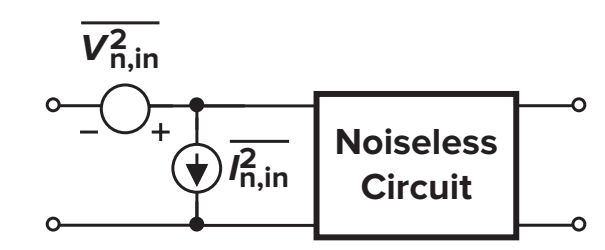
\includegraphics[width=0.27\linewidth]{../fig/ch7/fig7_33.png}\hspace{1.5em}
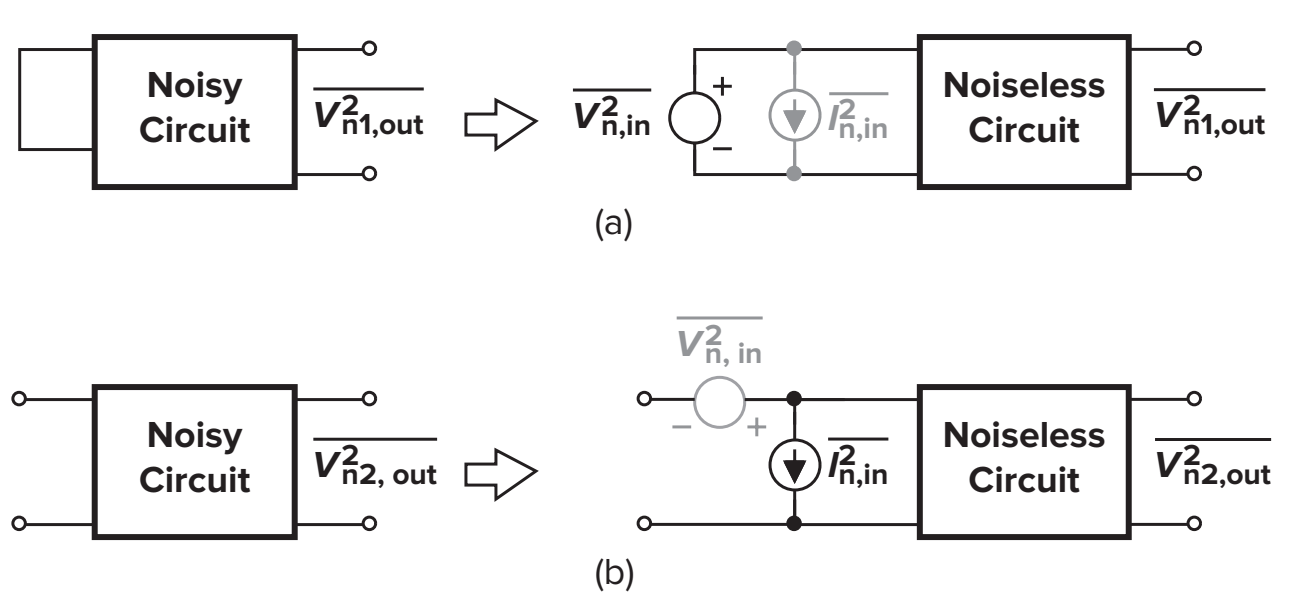
\includegraphics[width=0.52\linewidth]{../fig/ch7/fig7_34.png}\\[0.1em]
{\small\sffamily 圖 7.33\quad 電壓+電流源表示法（p.239）\qquad 圖 7.34\quad (a) 短路求 $\Vsq{in}$，(b) 開路求 $\Isq{in}$（p.239）}
\end{center}

\subsection{兩個極端源阻抗：短路求 $\Vsq{in}$、開路求 $\Isq{in}$ \lec{19}}
\begin{itemize}[leftmargin=2em]
  \item \textbf{輸入短路}（$Z_S=0$）：$\Isq{in}$ 被短路、不影響輸出，輸出雜訊全來自 $\Vsq{in}$。
  \item \textbf{輸入開路}（$Z_S=\infty$）：$\Vsq{in}$ 沒有電流可推、不影響輸出，輸出雜訊全來自 $\Isq{in}$。
\end{itemize}

\exhead{7.12}{239}{CS 級含 $C_{in}$ 的 $\Vsq{in}$ 與 $\Isq{in}$（只考慮熱雜訊）}
\rfig{35}{0.58}{輸入短路與輸入開路（p.240）}
短路時 $\Vsq{in}=4kT\gamma/g_m+4kT/(g_m^2R_D)$。開路時 $\Isq{in}$ 流過 $C_{in}$ 產生閘極電壓，令其輸出等於真實電路開路時的輸出：
\begin{align}
\Isq{in}\left(\frac{1}{C_{in}\omega}\right)^2g_m^2R_D^2=\left(4kT\gamma g_m+\frac{4kT}{R_D}\right)R_D^2
\ \Rightarrow\ \boxed{\Isq{in}=(C_{in}\omega)^2\frac{4kT}{g_m^2}\left(\gamma g_m+\frac1{R_D}\right)}
\end{align}
低頻時 $\Isq{in}\to0$，所以 MOS 閘極輸入的電路在低頻通常只需考慮 $\Vsq{in}$。

\textbf{何時可以忽略 $\Isq{in}$} \supp（課本 p.240，圖 7.36）：前級輸出阻抗為 $Z_S$ 時，本級輸入節點 $X$ 的雜訊為 $V_{n,X}=\frac{Z_{in}}{Z_{in}+Z_S}V_{n,in}+\frac{Z_{in}Z_S}{Z_{in}+Z_S}I_{n,in}$，因此
\begin{align}
\boxed{|Z_S|^2\ll\frac{\Vsq{in}}{\Isq{in}}}\ \Rightarrow\ \Isq{in}\ \text{可忽略}
\end{align}
決定 $I_{n,in}$ 重不重要的是\textbf{前級的輸出阻抗 $Z_S$}，不是本級的 $Z_{in}$。
\rfig{36}{0.3}{輸入雜訊電流的影響（p.240）}

\subsection{同時用 $V_{n,in}$ 與 $I_{n,in}$ 會不會把雜訊算兩次？\lec{20} \detail}
\rfig{37}{0.45}{由源阻抗 $Z_S$ 驅動的 CS 級（p.241）}
不會。關鍵是 $V_{n,in}$ 與 $I_{n,in}$ 來自同一批雜訊源、\textbf{高度相關}，必須用電壓（而非功率）疊加。由 \exref{7.12} 的兩個結果改寫成電壓形式（$V_{n,M1}$ 是 $M_1$ 的閘極參考雜訊、$V_{n,RD}$ 是 $R_D$ 的雜訊電壓）：
\begin{align}
V_{n,in}=V_{n,M1}+\frac{1}{g_mR_D}V_{n,RD},\qquad I_{n,in}=C_{in}s\,V_{n,M1}+\frac{C_{in}s}{g_mR_D}V_{n,RD}=C_{in}s\,V_{n,in}
\end{align}
節點 $X$ 的電壓（$V_{n,in}$ 經 $Z_S$、$1/(C_{in}s)$ 分壓，加上 $I_{n,in}$ 流過 $Z_S\parallel\frac1{C_{in}s}$）：
\begin{align}
V_{n,X}&=V_{n,in}\frac{1/(C_{in}s)}{1/(C_{in}s)+Z_S}+I_{n,in}\frac{Z_S/(C_{in}s)}{1/(C_{in}s)+Z_S}=\frac{V_{n,in}+I_{n,in}Z_S}{Z_SC_{in}s+1}\\
&=\frac{V_{n,in}(1+C_{in}sZ_S)}{Z_SC_{in}s+1}=V_{n,M1}+\frac{1}{g_mR_D}V_{n,RD}
\end{align}
與 $Z_S$、$C_{in}$ 都無關，故 $\Vsq{out}=g_m^2R_D^2\overline{V^2_{n,X}}=4kT\left(\gamma g_m+\frac1{R_D}\right)R_D^2$，正是真實電路的輸出雜訊，沒有重複計算。

\begin{trapbox}[常見陷阱：輸入參考雜訊的計算]
\begin{enumerate}[leftmargin=2.2em]
  \item \textbf{除以增益平方}：$\Vsq{in}=\Vsq{out}/A_v^2$，不是除以 $A_v$；$\Isq{in}$ 則除以「轉阻」的平方。
  \item \textbf{$V_{n,in}$ 與 $I_{n,in}$ 相關}：兩者同時作用（有限 $Z_S$）時不可直接把功率相加，要回到電壓疊加。
  \item \textbf{不能對 $\Vsq{in}$ 直接積分}：輸入參考頻譜常是白的（積分發散），總雜訊要在\textbf{輸出}積分後再除以中頻增益平方（7.9 節）。
  \item \textbf{$r_O$ 不產生雜訊}，但會影響轉移函數；題目給 $\lambda\neq0$ 時要用 $r_O$ 算輸出阻抗。
\end{enumerate}
\end{trapbox}

\exhead{7.13}{242}{含回授電阻 $R_F$ 的放大器（新電路、新方法：輸出短路電流法）\supp}
\rfig{38}{0.6}{回授電阻 $R_F$ 的放大器（p.242）}
有時先求\textbf{輸出短路雜訊電流}較簡單，再除以轉導 $G_m$（或電流增益）即得輸入參考雜訊。條件：$I_1$ 無雜訊、$\lambda=0$。
\begin{itemize}[leftmargin=2em]
  \item \textbf{求 $\Vsq{in}$}（輸入、輸出都短路，圖 b）：$R_F$ 兩端都是交流地，$\overline{I^2_{n1,out}}=4kT/R_F+4kT\gamma g_m$。轉導（圖 c）：$I_{out}=g_mV_{in}-V_{in}/R_F$，故 $G_m=g_m-1/R_F$，
  \[\Vsq{in}=\frac{4kT/R_F+4kT\gamma g_m}{(g_m-1/R_F)^2}\]
  \item \textbf{求 $\Isq{in}$}（輸入開路，圖 d）：$R_F$ 的雜訊電壓直接加在 $V_{GS}$ 上，$\overline{I^2_{n2,out}}=4kTR_Fg_m^2+4kT\gamma g_m$；電流增益（圖 e）：$I_{in}$ 流過 $R_F$ 使 $V_{GS}=I_{in}R_F$，$I_{out}=(g_mR_F-1)I_{in}$，
  \[\Isq{in}=\frac{4kTR_Fg_m^2+4kT\gamma g_m}{(g_mR_F-1)^2}\]
\end{itemize}
新觀察：此電路輸入短路與開路時的輸出雜訊不同，所以 $\Isq{in}$ 不可忽略（對照附錄 A：只有輸出雜訊幾乎不隨 $Z_S$ 改變的電路才能省掉 $I_{n,in}$）。

\subsection{Lemma：汲極雜訊電流 $\Leftrightarrow$ 閘極雜訊電壓 \lec{21} \detail}
\rfig{39}{0.7}{等效的兩個 CS 級（p.244）}
\textbf{Lemma}：低頻下，若 $\overline{V_n^2}=\overline{I_n^2}/g_m^2$，則圖 (a)、(b) 兩電路對\textbf{任意} $Z_S$ 都等效。

\textbf{證明}（講義手寫）：兩電路輸出阻抗相同，只需比較\textbf{輸出短路電流}（圖 c、d）。對 (c)，設源極電壓 $V_S$，則 $V_{gs}=-V_S$，且源極電流全部流過 $Z_S$：$V_S=I_{n,out}Z_S$。在汲極節點寫 KCL：
\begin{align}
I_{n,out}&=g_mV_{gs}-g_{mb}V_S-\frac{V_S}{r_O}+I_n=-\Big(g_m+g_{mb}+\frac1{r_O}\Big)V_S+I_n\\
&=-\Big(g_m+g_{mb}+\frac1{r_O}\Big)Z_SI_{n,out}+I_n
\ \Rightarrow\ I_{n,out1}=\frac{I_n}{Z_S(g_m+g_{mb}+1/r_O)+1}
\end{align}
同理 (d) 中 $V_n$ 相當於把 $V_{gs}$ 多加 $V_n$，得
\[I_{n,out2}=\frac{g_mV_n}{Z_S(g_m+g_{mb}+1/r_O)+1}\]兩者相等 $\Leftrightarrow\boxed{V_n=I_n/g_m}$，與 $Z_S$ 無關。$V_n$ 稱為 $M_1$ 的\textbf{閘極參考雜訊}。

\textbf{用法}：把每顆電晶體的雜訊直接寫成串在閘極的 $4kT\gamma/g_m+K/(C_{ox}WLf)$，再乘上「從那顆電晶體的閘極到輸出的增益」，是單級電路最快的解法。

\exhead{7.14}{244}{用 Thevenin 等效證明 lemma \supp}
\rfig{40}{0.7}{以 Thevenin 等效比較兩電路（p.245）}
把 $Z_L$ 以外的部分化成 Thevenin 等效。$I_n=V_n=0$ 時兩電路相同，故 $Z_{Thev1}=Z_{Thev2}$，只需比較 Thevenin 電壓。求 Thevenin 電壓時 $Z_L$ 開路（圖 c），汲極沒有電流，$Z_S$ 上也沒有電流，所以 $V_{Thev1}=I_nr_O$、$V_{Thev2}=g_mV_nr_O$，同樣得 $V_n=I_n/g_m$。

% =====================================================================
\section{單級放大器的雜訊}

\subsection{Common-source 級：放大用的電晶體要 $g_m$ 大 \lec{22}}
\begin{align}
\Vsq{in}=4kT\left(\frac{\gamma}{g_m}+\frac{1}{g_m^2R_D}\right)+\frac{K}{C_{ox}WL}\frac1f
\end{align}
電晶體放大閘極電壓訊號時 $g_m$ 要大；當定電流源時 $g_m$ 要小（課本圖 7.41）。降低雜訊的兩個方向與代價（講義手寫）：
\begin{enumerate}[leftmargin=2em]
  \item \textbf{提高 $I_D$ 或 $W$}：$g_m\uparrow$，代價是功耗、寄生電容與 headroom。代入 $g_m=2I_D/V_{ov}$：
  \[\Vsq{in,th}=4kT\left[\frac{\gamma V_{ov}}{2I_D}+\frac{V_{ov}^2}{4I_D\cdot I_DR_D}\right]\]
  固定 $I_DR_D$（headroom）與 $V_{ov}$（$W\propto I_D$）時，$I_D\uparrow\Rightarrow\Vsq{in}\downarrow$，代價是功耗。
  \item \textbf{提高 $R_D$}：$\Vsq{in}\downarrow$，代價是 headroom 與速度下降。
\end{enumerate}

\exhead{7.15}{245}{電流源負載 CS 級的雜訊與輸出 SNR（重要新觀察：$g_{m1}$ 大、$g_{m2}$ 小）\lec{22--23}}
\rfig{42}{0.5}{電流源負載 CS 級（p.246）}
兩顆電晶體的雜訊電流都流過 $r_{O1}\parallel r_{O2}$：
\begin{align}
\Vsq{out}&=4kT\gamma(g_{m1}+g_{m2})(r_{O1}\parallel r_{O2})^2,\qquad A_v=g_{m1}(r_{O1}\parallel r_{O2})\\
\Vsq{in}&=4kT\gamma\left(\frac{1}{g_{m1}}+\frac{g_{m2}}{g_{m1}^2}\right)
\end{align}
直觀：$g_{m1}\uparrow$ 時輸出雜訊電壓 $\propto\sqrt{g_{m1}}$、增益 $\propto g_{m1}$，所以輸入雜訊下降；$M_2$ 不放大訊號，沒有這個好處，因此希望 $g_{m2}$ 小。

\textbf{輸出 SNR}（講義 p.23）：接上 $C_L$ 後，輸出頻譜被 $r_{O1}\parallel r_{O2}$ 與 $C_L$ 低通，套用 $kT/C$ 的積分：
\begin{align}
\Vsq{out,tot}&=\int_0^\infty\frac{4kT\gamma(g_{m1}+g_{m2})(r_{O1}\parallel r_{O2})^2\,df}{1+(r_{O1}\parallel r_{O2})^2C_L^2(2\pi f)^2}=\gamma(g_{m1}+g_{m2})(r_{O1}\parallel r_{O2})\frac{kT}{C_L}\\
\text{SNR}_{out}&=\frac{\left[g_{m1}(r_{O1}\parallel r_{O2})V_m/\sqrt2\right]^2}{\gamma(g_{m1}+g_{m2})(r_{O1}\parallel r_{O2})(kT/C_L)}=\frac{C_L}{2\gamma kT}\cdot\frac{g_{m1}^2(r_{O1}\parallel r_{O2})}{g_{m1}+g_{m2}}V_m^2
\end{align}
$C_L\uparrow\Rightarrow$ SNR$\uparrow$ 但頻寬$\downarrow$：寬頻又低雜訊的電路很難設計。

\exhead{7.16}{247}{互補 CS 級（新電路）\supp}
\rfig{43}{0.12}{互補 CS 級（p.247）}
輸入設為零時，輸出雜訊與 \exref{7.15} 相同；但兩顆都在放大輸入，增益變成 $(g_{m1}+g_{m2})(r_{O1}\parallel r_{O2})$：
\begin{align}
\boxed{\Vsq{in}=\frac{4kT\gamma}{g_{m1}+g_{m2}}}
\end{align}
好比兩顆並聯、轉導相加。比電流源負載 CS 低雜訊的原因：$M_2$ 一樣注入雜訊，但在這裡它同時也是轉導元件、會放大訊號。

\exhead{7.17}{247}{電流源負載再並聯 $R_D$ 的 CS 級（含 $1/f$）\supp}
\rfig{44}{0.5}{電流源負載與電阻並聯（p.247）}
$M_2$ 的閘極雜訊經 $g_{m2}(R_D\parallel r_{O1}\parallel r_{O2})$ 到輸出，再除以主增益 $g_{m1}(R_D\parallel r_{O1}\parallel r_{O2})$：
\begin{align}
\Vsq{in}=4kT\gamma\left(\frac{1}{g_{m1}}+\frac{g_{m2}}{g_{m1}^2}\right)+\frac{1}{C_{ox}f}\left[\frac{K_N}{(WL)_1}+\frac{K_Pg_{m2}^2}{(WL)_2g_{m1}^2}\right]+\frac{4kT}{g_{m1}^2R_D}
\end{align}
$R_D=\infty$ 時退化成\exref{7.15}，$g_{m2}=0$ 時退化成電阻負載 CS。

\exhead{7.18}{248}{flicker 雜訊電流「與 $W$ 無關」？（觀念陷阱）\supp}
把汲極 $1/f$ 雜訊電流寫成 $\frac{K}{WLC_{ox}f}\cdot2\mu_nC_{ox}\frac WL I_D=\frac{2K\mu_nI_D}{L^2f}$，就會誤以為與 $W$ 無關。公平比較要同時固定 $I_D$ \textbf{與} overdrive（否則 headroom 也變了），應寫成 $\frac{K}{WLC_{ox}f}\cdot\frac{4I_D^2}{V_{ov}^2}$，可見面積越大雜訊越小。

\exhead{7.19}{248}{電阻負載 CS 級的雜訊設計（設計題）\supp}
\rfig{45}{0.5}{CS 級的總雜訊設計（p.249）}
規格：總輸入參考雜訊 $100\,\mu\text{V}_{\text{rms}}$、功耗 1\,mW、頻寬 1\,GHz（由 $R_D$ 與 $C_L$ 決定）、$V_{DD}=1$\,V，忽略 $\lambda$ 與 $1/f$。
\begin{align}
\Vsq{out}&=(1+\gamma g_mR_D)\frac{4kTR_D}{R_D^2C_L^2\omega^2+1}\ \Rightarrow\ \Vsq{out,tot}=(1+\gamma g_mR_D)\frac{kT}{C_L}\\
\Vsq{in,tot}&=\frac{1+\gamma g_mR_D}{g_m^2R_D^2}\cdot\frac{kT}{C_L}=\frac{1+\gamma g_mR_D}{g_m^2R_D}\cdot2\pi kT\cdot\underbrace{\frac{1}{2\pi R_DC_L}}_{1\,\text{GHz}}=(100\,\mu\text{V})^2\\
&\Rightarrow\ \frac1{g_m}\left(\frac{1}{g_mR_D}+\gamma\right)=\frac{(100\,\mu\text{V})^2}{2\pi kT\times1\,\text{GHz}}=384\,\Omega
\end{align}
取 $g_mR_D=3$、$\gamma=1$：$1/g_m=288\,\Omega$、$R_D=864\,\Omega$；$I_D=1$\,mA 時 $I_DR_D=864$\,mV，只剩 $V_{DS}=136$\,mV，擺幅很小（可改試 $g_mR_D=2$ 或 4 比較 headroom）。

\subsection{Common-gate 級：負載雜訊直接成為輸入雜訊電流 \lec{24}}
\begin{center}
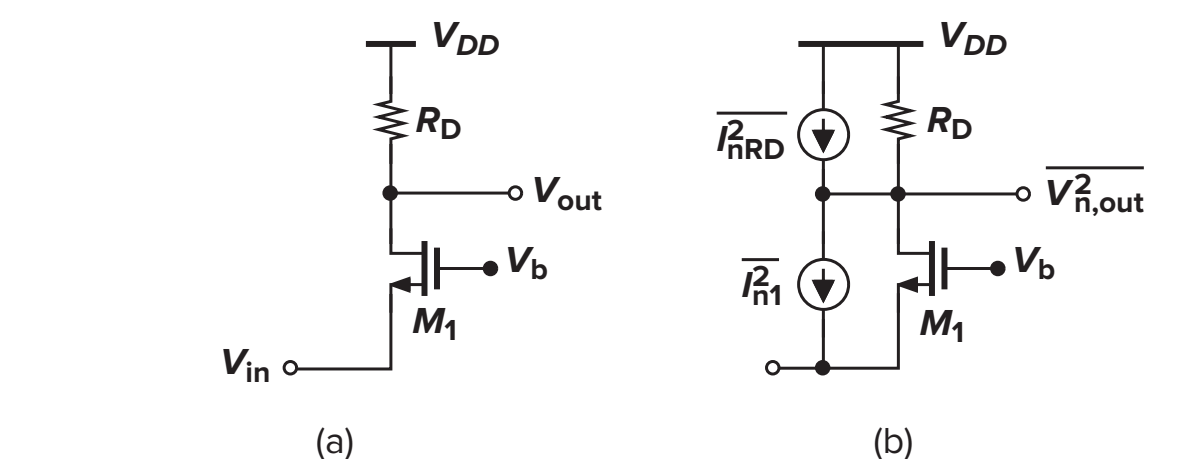
\includegraphics[width=0.36\linewidth]{../fig/ch7/fig7_46.png}\hspace{1em}
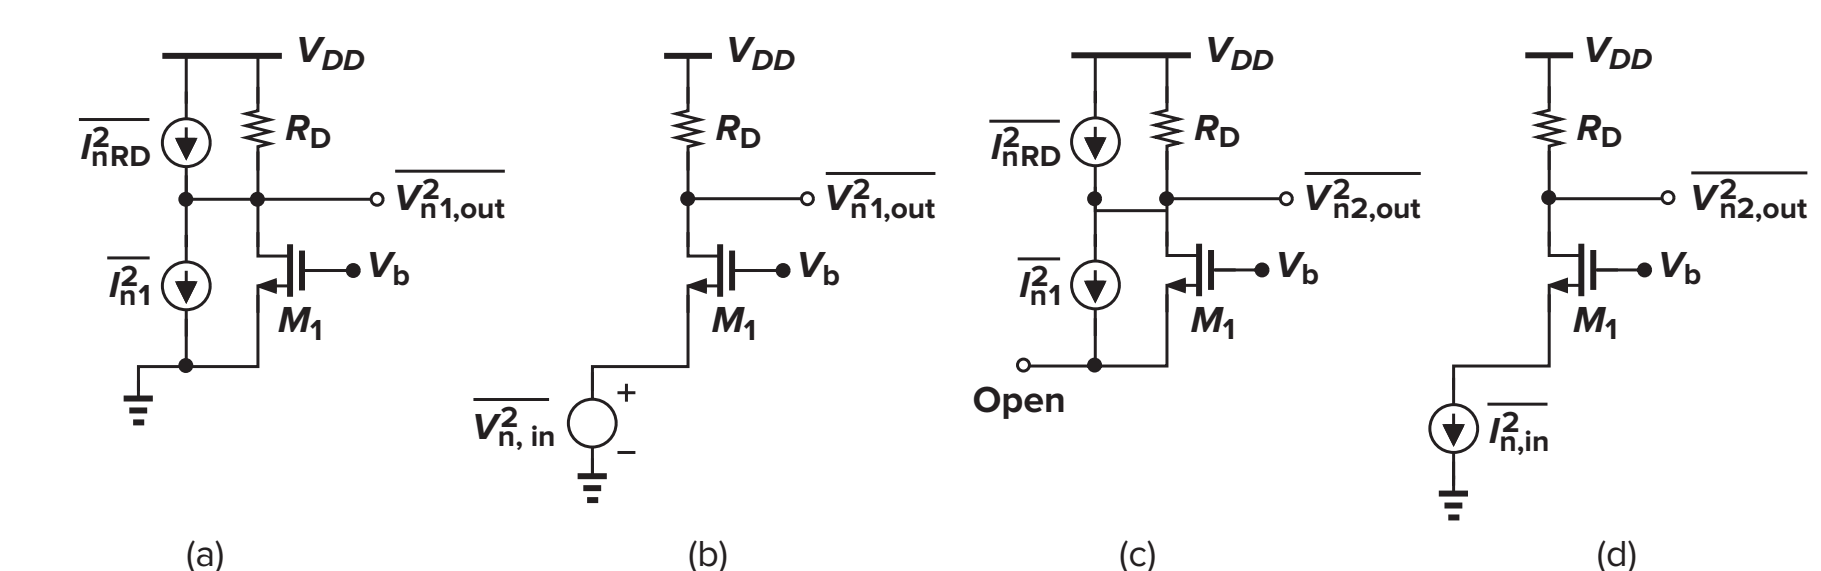
\includegraphics[width=0.56\linewidth]{../fig/ch7/fig7_47.png}\\[0.1em]
{\small\sffamily 圖 7.46\quad CG 級與雜訊源\qquad 圖 7.47\quad (a)(b) 短路求 $\Vsq{in}$；(c)(d) 開路求 $\Isq{in}$（p.250）}
\end{center}
CG 輸入阻抗低，\textbf{即使在低頻 $\Isq{in}$ 也不可忽略}。
\begin{itemize}[leftmargin=2em]
  \item \textbf{輸入短路}：$\left(4kT\gamma g_m+\frac{4kT}{R_D}\right)R_D^2=\Vsq{in}(g_m+g_{mb})^2R_D^2$，
  \[\Vsq{in}=\frac{4kT(\gamma g_m+1/R_D)}{(g_m+g_{mb})^2}\]
  \item \textbf{輸入開路} \detail：源極節點沒有其他路徑，KCL 給 $I_{n1}+I_{D1}=0$，也就是 $M_1$ 的雜訊電流只在元件內部循環，\textbf{對輸出沒有貢獻}；輸出雜訊只剩 $4kTR_D$。令 $\Isq{in}$（全部流過 $M_1$ 到 $R_D$，電流增益 1）產生同樣的輸出：
  \[\Isq{in}R_D^2=4kTR_D\ \Rightarrow\ \boxed{\Isq{in}=\frac{4kT}{R_D}}\]
\end{itemize}
\textbf{缺點}：CG 沒有電流增益，負載的雜訊電流被原封不動地參考回輸入。

\subsection{偏壓電流源的雜訊 \lec{25}}
\rfig{48}{0.3}{偏壓電流源 $M_2$ 的雜訊（p.251）}
\begin{itemize}[leftmargin=2em]
  \item \textbf{輸入短路}：$M_2$ 的雜訊電流被短路到地，不流過 $R_D$，對 $\Vsq{in}$ 無貢獻。
  \item \textbf{輸入開路}：$I_{n2}$ 全部流經 $M_1$、$R_D$，所以 $\overline{I^2_{n2}}$ \textbf{直接加到 $\Isq{in}$}。
\end{itemize}
要讓 $g_{m2}=2I_{D2}/V_{ov2}$ 小，給定電流時需大 overdrive，會吃掉 $V_b$ 的空間並限制輸出擺幅。$M_0$ 的雜訊由 $C_0$ 濾掉（講義手寫）。

\exhead{7.20}{251}{PMOS 電流源負載的 CG 級：熱雜訊與 flicker 雜訊 \lec{26}}
\begin{center}
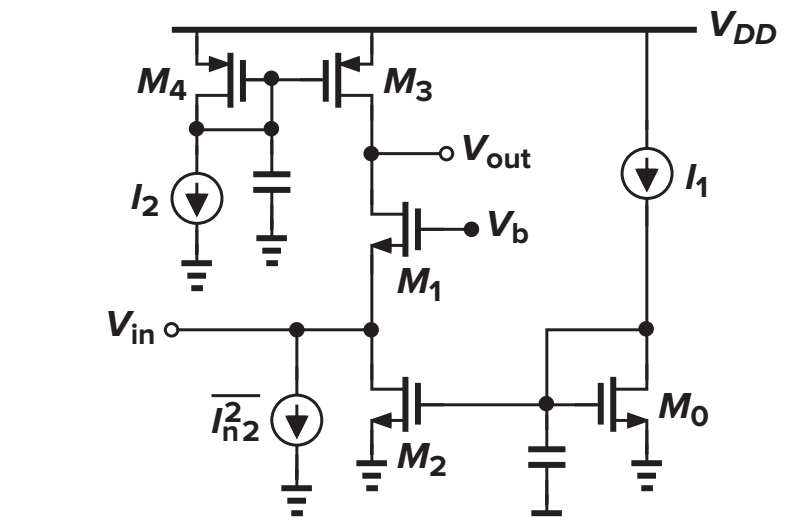
\includegraphics[width=0.28\linewidth]{../fig/ch7/fig7_49.png}\hspace{2em}
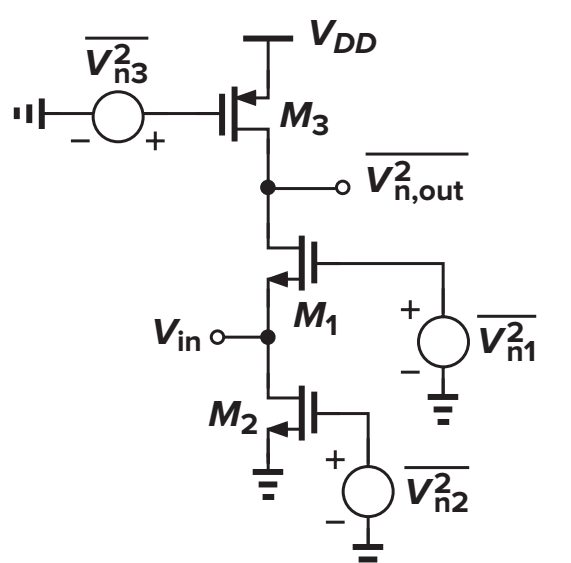
\includegraphics[width=0.22\linewidth]{../fig/ch7/fig7_50.png}\\[0.1em]
{\small\sffamily 圖 7.49\quad 電路（p.251）\qquad 圖 7.50\quad 各管 $1/f$ 雜訊串在閘極（p.252）}
\end{center}
講義 p.26 只列 flicker 雜訊；課本例題先算熱雜訊，這裡一併整理。全部飽和，忽略 $M_0$、$M_4$ 的雜訊。

\textbf{熱雜訊} \supp：
\begin{itemize}[leftmargin=2em]
  \item \textbf{輸入短路}：$M_2$ 被短路，$M_1$、$M_3$ 的雜訊電流流過 $r_{O1}\parallel r_{O3}$，增益約 $(g_{m1}+g_{mb1})(r_{O1}\parallel r_{O3})$：
  \[\Vsq{in}=4kT\gamma\frac{g_{m1}+g_{m3}}{(g_{m1}+g_{mb1})^2}\]
  \item \textbf{輸入開路}：$M_2$ 的雜訊電流直接加到輸入；$M_3$ 的雜訊參考回輸入時，在任何 $g_mr_O\gg1$ 下 $I_{n,in}|_{M3}\approx I_{n3}$；$M_1$ 的雜訊因源極看到 $r_{O2}$ 這麼大的退化而可忽略。
  \[\Isq{in}=4kT\gamma(g_{m2}+g_{m3})\]
\end{itemize}
兩者都正比於\textbf{電流源}電晶體的 $g_m$。

\textbf{Flicker 雜訊}（講義 p.26）：輸入短路時，$M_1$、$M_3$ 的閘極源經各自的轉導到輸出，再除以增益 $(g_{m1}+g_{mb1})(r_{O1}\parallel r_{O3})$；輸入開路時 $M_1$ 因 $r_{O2}$ 很大而無貢獻，$M_2$、$M_3$ 的閘極源各乘 $g_m$ 成為輸入電流：
\begin{align}
\Vsq{in}=\frac{1}{C_{ox}f}\left[\frac{g_{m1}^2K_N}{(WL)_1}+\frac{g_{m3}^2K_P}{(WL)_3}\right]\frac{1}{(g_{m1}+g_{mb1})^2},\qquad
\Isq{in}=\frac{1}{C_{ox}f}\left[\frac{g_{m2}^2K_N}{(WL)_2}+\frac{g_{m3}^2K_P}{(WL)_3}\right]
\end{align}
總雜訊為熱雜訊與 flicker 雜訊相加。

\subsection{Source follower：增益小於 1 卻加雜訊 \lec{27}}
\rfig{51}{0.45}{(a) Source follower；(b) 含雜訊源（p.253）}
輸入阻抗高，通常忽略 $\Isq{in}$。$M_2$ 的雜訊電流看到的阻抗是 $R_{out}=\frac1{g_{m1}}\parallel\frac1{g_{mb1}}\parallel r_{O1}\parallel r_{O2}$：
\begin{align}
\Vsq{out}|_{M2}=\overline{I^2_{n2}}\left(\frac1{g_{m1}}\Big\|\frac1{g_{mb1}}\Big\|r_{O1}\|r_{O2}\right)^2,\qquad
A_v=\frac{\frac1{g_{mb1}}\|r_{O1}\|r_{O2}}{\frac1{g_{mb1}}\|r_{O1}\|r_{O2}+\frac1{g_{m1}}}<1
\end{align}
$A_v^2$ 的分母正好讓 $R_{out}^2/A_v^2=1/g_{m1}^2$，故
\begin{align}
\Vsq{in}=\overline{V^2_{n1}}+\frac{\Vsq{out}|_{M2}}{A_v^2}=4kT\gamma\left(\frac1{g_{m1}}+\frac{g_{m2}}{g_{m1}^2}\right)
\end{align}
形式與電流源負載 CS 相同。只加雜訊、增益又小於 1，所以\textbf{低雜訊放大鏈中盡量避免 SF}。

\subsection{Cascode 級：低頻時 cascode 管幾乎不貢獻 \lec{28} \detail}
\rfig{52}{0.5}{(a) Cascode；(b)(c) $M_2$ 的雜訊模型（p.254）}
低頻下 $M_1$、$R_D$ 的貢獻與 CS 相同：$\Vsq{in}|_{M1,R_D}=4kT\left(\frac{\gamma}{g_{m1}}+\frac{1}{g_{m1}^2R_D}\right)$。

\textbf{$M_2$ 為何可忽略}（講義手寫）：
\begin{itemize}[leftmargin=2em]
  \item 電流源觀點（圖 b）：若 $r_{O1}=\infty$，$X$ 點只能流 $M_1$ 的電流，$I_{n2}+I_{D2}=0$，$M_2$ 的雜訊電流在內部循環，輸出雜訊為零。
  \item 電壓源觀點（圖 c）：$M_2$ 相當於源極退化 $r_{O1}$ 的 CS 級，等效轉導 $g_{m,eff}=\dfrac{g_{m2}}{1+g_{m2}r_{O1}}$，
  \[\frac{V_{n,out}}{V_{n2}}=\frac{g_{m2}R_D}{1+g_{m2}r_{O1}}\approx\frac{R_D}{r_{O1}}\ll1\]
  （若負載是 PMOS cascode 這類大阻抗，$R_D\sim g_mr_O^2$，此增益約 $g_mr_O$，就不能忽略。）
\end{itemize}
\textbf{高頻}：$X$ 點電容 $C_X$ 讓 $V_{n2}$ 到輸出的增益變成 $\frac{V_{n,out}}{V_{n2}}\approx\frac{-R_D}{1/g_{m2}+1/(C_Xs)}$，隨頻率上升；同時 $C_X$ 分流 $M_1$ 的訊號電流、主增益下降。兩者疊加，cascode 的輸入參考雜訊在高頻會明顯惡化。

% =====================================================================
\section{電流鏡的雜訊：二極體接法元件的雜訊被放大 $N$ 倍}
\subsection{以 $C_B$ 濾除 $M_{REF}$ 的雜訊 \lec{29}}
\rfig{53}{0.72}{(a) 以 $C_B$ 抑制 $M_{REF}$ 雜訊的電流鏡；(b) 小訊號模型；(c) 等效電路（p.255）}
$(W/L)_1=N(W/L)_{REF}$。$M_{REF}$ 與其雜訊的 Thevenin 等效 \detail：開路電壓就是 $V_{n,REF}$（$I_{REF}$ 為理想電流源，圖 b 中 $g_{m,REF}V_1$ 必須為零，即 $V_1=0$），內阻 $1/g_{m,REF}$。它與 $C_B$ 構成低通，$X$ 點電壓
\begin{align}
V_X=\frac{1/(sC_B)}{1/g_{m,REF}+1/(sC_B)}V_{n,REF}=\frac{g_{m,REF}}{g_{m,REF}+sC_B}V_{n,REF}
\end{align}
與 $M_1$ 自己的 $V_{n1}$ 一起驅動 $M_1$：
\begin{align}
\Isq{out}=\left(\frac{g_{m,REF}^2}{C_B^2\omega^2+g_{m,REF}^2}\overline{V^2_{n,REF}}+\overline{V^2_{n1}}\right)g_{m1}^2
\end{align}
同 $L$ 時面積比為 $N$，$1/f$ 雜訊 $\propto1/(WL)$，故 $\overline{V^2_{n,REF}}=N\overline{V^2_{n1}}$：
\begin{align}
\Isq{out}=\left(\frac{N\,g_{m,REF}^2}{C_B^2\omega^2+g_{m,REF}^2}+1\right)g_{m1}^2\overline{V^2_{n1}},\qquad
\text{可忽略條件：}\ \boxed{C_B^2\gg\frac{(N-1)g_{m,REF}^2}{\omega^2}}
\end{align}
數值（課本）：$N=5$、$g_{m,REF}=1/(200\,\Omega)$、最低頻 1\,MHz $\Rightarrow C_B\gg1.59$\,nF；要十倍抑制需 5.03\,nF，晶片上不切實際（講義：$C_B\sim$\,nF）。

\subsection{串入 $R_B$ 降低截止頻率 \lec{30}}
\rfig{54}{0.5}{(a) 在閘極串 $R_B$；(b) 以 MOS $M_R$ 實現大電阻（p.256）}
截止頻率降為 $\omega_c=\dfrac{g_{m,REF}}{(1+g_{m,REF}R_B)C_B}=\dfrac{1}{(R_B+1/g_{m,REF})C_B}$：
\begin{align}
\Isq{out}=\left[\frac{g_{m,REF}^2}{(1+g_{m,REF}R_B)^2C_B^2\omega^2+g_{m,REF}^2}\left(\overline{V^2_{n,REF}}+\overline{V^2_{n,R_B}}\right)+\overline{V^2_{n1}}\right]g_{m1}^2
\end{align}
$R_B$ 本身有熱雜訊，但只要 $\overline{V^2_{n,R_B}}$ 仍小於 $M_{REF}$ 的 $1/f$ 雜訊，就能把 $R_B$ 做得很大；上限還受閘極漏電流造成的 dc 誤差限制。實作上 $R_B$ 用小 overdrive 的 MOS $M_R$（$L$ 大、$W$ 小），並用 $M_C$（$L$ 小、$W$ 大）提供偏壓。

% =====================================================================
\section{差動對的雜訊：輸入參考雜訊功率是 CS 的 2 倍}

\subsection{電阻負載差動對 \lec{31--33} \detail}
\rfig{56}{0.55}{差動對可視為二埠電路；輸入參考雜訊的計算（p.257）}
差動對可視為差動輸入、差動輸出的二埠電路；輸入阻抗高，低頻時 $\Isq{in}$ 可忽略。$I_{n1}$ 與 $I_{n2}$ 不相關，$P$ 點\textbf{不是}虛接地（雜訊源不是差動訊號），不能用半電路，只能逐一計算（忽略 $r_O$）。

\textbf{$I_{n1}$ 的分流}（講義手寫）：兩管 $V_{GS}$ 相同（閘極接地、源極相連），故 $g_m v_{gs1}=g_mv_{gs2}=g_mv_{gs}$。$P$ 點 KCL：$M_1$ 的總電流與 $M_2$ 的電流必須互相抵消（尾電流源對雜訊開路），
\begin{align}
g_mv_{gs}+I_{n1}=-g_mv_{gs}\ \Rightarrow\ g_mv_{gs}=-\frac{I_{n1}}{2}
\end{align}
所以 $I_{n1}$ 一半流經 $R_{D1}$、一半經 $M_2$ 流經 $R_{D2}$，兩端電壓反相，差動輸出為兩者相加（同源，電壓相加）：
\begin{align}
V_{n,out}|_{M1}&=\frac{I_{n1}}{2}R_{D1}+\frac{I_{n1}}{2}R_{D2}\ \xrightarrow{R_{D1}=R_{D2}=R_D}\ \Vsq{out}|_{M1}=\overline{I^2_{n1}}R_D^2\\
\Vsq{out}&=\left(\overline{I^2_{n1}}+\overline{I^2_{n2}}\right)R_D^2+2(4kTR_D)=8kT(\gamma g_mR_D^2+R_D)\\
\Vsq{in}&=\frac{\Vsq{out}}{g_m^2R_D^2}=\boxed{8kT\left(\frac{\gamma}{g_m}+\frac{1}{g_m^2R_D}\right)}
\end{align}
\rfig{57}{0.36}{用 lemma：每管雜訊串在閘極（p.258）}
\textbf{用 lemma 更快} \lec{32}：兩管各串 $\overline{V^2_{n1}}=\overline{V^2_{n2}}=4kT\gamma/g_m$，$R_{D1}$、$R_{D2}$ 的雜訊各除以 $g_m^2R_D^2$，直接得到上式。加入 $1/f$：
\begin{align}
\Vsq{in,tot}=8kT\left(\frac{\gamma}{g_m}+\frac{1}{g_m^2R_D}\right)+\frac{2K}{C_{ox}WL}\frac1f=2\,\Vsq{in,CS}
\end{align}
\textbf{結論}：每管 $g_m$ 相同時，差動對的輸入參考雜訊\textbf{功率}是 CS 的 2 倍（電壓為 $\sqrt2$ 倍），因為訊號路徑上的元件數加倍；一般而言，\textbf{全差動電路的 $\Vsq{in}$ = 半電路的 2 倍}。

\subsection{尾電流源的雜訊 \lec{34} \detail}
\rfig{55}{0.7}{尾電流源雜訊的影響（p.258）}
輸入差動為零且完全對稱時，$I_{SS}$ 的雜訊平分到兩邊，只產生共模雜訊。輸入有小差動 $\Delta V_{in}$ 時，雜訊 $I_n$ 會\textbf{調變每顆電晶體的轉導}：
\begin{align}
\Delta I_{D1}-\Delta I_{D2}&=g_m\Delta V_{in}=\sqrt{2\mu_nC_{ox}\frac WL\cdot\frac{I_{SS}+I_n}{2}}\;\Delta V_{in}
=\sqrt{2\mu_nC_{ox}\frac WL\cdot\frac{I_{SS}}{2}}\sqrt{1+\frac{I_n}{I_{SS}}}\;\Delta V_{in}\\
&\approx g_{m0}\left(1+\frac{I_n}{2I_{SS}}\right)\Delta V_{in}\qquad(\text{用 }\sqrt{1+x}\approx1+x/2,\ I_n\ll I_{SS})
\end{align}
雜訊項 $g_{m0}\frac{I_n}{2I_{SS}}\Delta V_{in}$ 與 $\Delta V_{in}$ 成正比、且 $I_n\ll I_{SS}$，通常可忽略。

\exhead{7.21}{259}{次臨界差動對做成浮接大電阻（新電路）\supp}
\rfig{58}{0.42}{(a) 電流源負載差動對做成浮接電阻；(b) 半電路（p.259）}
把 $M_1$、$M_2$ 偏在極小電流，$A$、$B$ 之間呈現約 $1/g_{m1}+1/g_{m2}=2/g_{m1}$ 的大增量電阻。用半電路（圖 b）求 $A$ 點的 Thevenin 雜訊：$M_1$ 是二極體接法、阻抗 $1/g_{m1}$，$M_1$、$M_3$ 的雜訊電流都流過它；$M_3$ 的 $1/f$ 閘極源乘 $g_{m3}/g_{m1}$：
\begin{align}
\overline{V^2_{n,A}}&=(4kT\gamma g_{m1}+4kT\gamma g_{m3})\frac{1}{g_{m1}^2}+\frac{K}{(WL)_1C_{ox}f}+\frac{K}{(WL)_3C_{ox}f}\left(\frac{g_{m3}}{g_{m1}}\right)^2\\
\overline{V^2_{n,AB}}&=2\overline{V^2_{n,A}}=8kT\gamma(g_{m1}+g_{m3})\frac{1}{g_{m1}^2}+\frac{2K}{(WL)_1C_{ox}f}+\frac{2K}{(WL)_3C_{ox}f}\left(\frac{g_{m3}}{g_{m1}}\right)^2
\end{align}
新觀察：同阻值（$2/g_{m1}$）的歐姆電阻只有 $4kT\cdot2/g_{m1}=8kT/g_{m1}$，這個「電阻」多了 $\gamma$、$M_3$ 與 $1/f$ 的貢獻，所以更吵，也更不線性。

\exhead{7.22}{260}{電流源負載差動對的輸入參考雜訊（新電路、新方法）\supp}
\rfig{59}{0.5}{(a) 電流源負載差動對；(b) 雜訊源；(c) $M_3$ 雜訊電流的分流（p.260）}
$M_1$、$M_2$ 的雜訊已是輸入串聯源，只需把 $M_3$、$M_4$ 參考到輸入。$M_3$ 的雜訊電流 $g_{m3}V_{n3}$ 分流到 $r_{O3}$ 與看入 $M_1$ 汲極的 $R_X=r_{O4}+2r_{O1}$：
\begin{align}
I_{nA}=g_{m3}V_{n3}\frac{r_{O4}+2r_{O1}}{2r_{O4}+2r_{O1}},\qquad I_{nB}=g_{m3}V_{n3}\frac{r_{O3}}{2r_{O4}+2r_{O1}}
\end{align}
$V_{nX}=-I_{nA}r_{O3}$、$V_{nY}=I_{nB}r_{O4}$，相減（$V_{nY}$ 要從 $V_{nX}$ 減掉）得
\begin{align}
V_{nXY}=V_{nX}-V_{nY}=g_{m3}V_{n3}\frac{r_{O3}r_{O1}}{r_{O3}+r_{O1}}
\end{align}
即 $M_3$ 的雜訊電流乘上 $r_{O1}\parallel r_{O3}$。
\rfig{60}{0.62}{另一種看法：把 $V_{n3}$ 拆成兩個差動分量，再用半電路（p.261）}
\textbf{新方法}：雖然雜訊是隨機的，但只有一個雜訊源時可以暫時把它當成確定性訊號，拆成 $\pm V_{n3}/2$ 的差動分量施加在 $M_3$、$M_4$ 閘極，再用半電路，得到相同結果。$M_4$ 同理，功率相加後除以 $g_{m1}^2(r_{O1}\parallel r_{O3})^2$：
\begin{align}
\Vsq{in}=2\overline{V^2_{n1}}+2\frac{g_{m3}^2}{g_{m1}^2}\overline{V^2_{n3}}
=8kT\gamma\left(\frac1{g_{m1}}+\frac{g_{m3}}{g_{m1}^2}\right)+\frac{2K_N}{C_{ox}(WL)_1f}+\frac{2K_P}{C_{ox}(WL)_3f}\frac{g_{m3}^2}{g_{m1}^2}
\end{align}

\subsection{五電晶體 OTA \lec{35} \detail}
\rfig{61}{0.28}{求輸出短路雜訊電流（p.262）}
OTA 不對稱，改求 Norton 等效（輸出短路電流 $\Isq{out}$），再乘 $R_{out}$ 得輸出電壓、除以增益 $A_v=G_mR_{out}$。$G_m\approx g_{m1,2}$，$R_{out}\approx r_{O1,2}\parallel r_{O3,4}$。逐顆計算（講義手寫）：
\begin{itemize}[leftmargin=2em]
  \item $M_1$、$M_2$：各自的閘極雜訊 $4kT\gamma/g_{m1,2}$ 乘 $g_{m1,2}^2$：$\overline{I^2_{n1,out}}+\overline{I^2_{n2,out}}=2\cdot4kT\gamma g_{m1,2}$。
  \item $M_3$：雜訊電流 $I_{n3}$ 主要流過二極體阻抗 $1/g_{m3}$，在 $M_4$ 閘極產生 $I_{n3}/g_{m3}$，再乘 $g_{m4}$ 出現在輸出：$\overline{I^2_{n3,out}}=\frac{g_{m4}^2}{g_{m3}^2}4kT\gamma g_{m3}=4kT\gamma g_{m3,4}$（$g_{m3}=g_{m4}$）。
  \item $M_4$：雜訊電流直接流入短路：$\overline{I^2_{n4,out}}=4kT\gamma g_{m4}$。
\end{itemize}
\begin{align}
\Isq{out}=4kT\gamma(2g_{m1,2}+2g_{m3,4}),\qquad
\Vsq{in}=\frac{\Isq{out}R_{out}^2}{g_{m1,2}^2R_{out}^2}=8kT\gamma\left(\frac1{g_{m1,2}}+\frac{g_{m3,4}}{g_{m1,2}^2}\right)
\end{align}
與全差動的電流源負載差動對（\exref{7.22}）相同。

\subsection{OTA 中尾電流源的雜訊會出現在輸出 \lec{36} \detail}
\rfig{62}{0.24}{尾電流雜訊的影響（p.262）}
$V_{out}$ 跟隨 $V_X$（輸入相同、電路對稱時，$V_{out}=V_X$）。$I_{SS}$ 的雜訊平分，$I_n/2$ 流過二極體 $M_3$ 的阻抗 $1/g_{m3}$：
\begin{align}
\overline{V^2_{n,X}}=\left(\frac{I_n}{2}\right)^2\frac{1}{g_{m3}^2}=\Vsq{out}
\end{align}
在全差動電路中尾電流雜訊只是共模；但 5T OTA 是單端輸出，它會直接出現在輸出端。

% =====================================================================
\section{雜訊–功耗取捨：雜訊功率減半需付出兩倍功耗}
\rfig{63}{0.55}{(a) 以縮放降低雜訊；(b) 等效為兩電路並聯；(c) 佈局觀點（p.263）}
\lec{37}：把 $W$ 與 $I_D$ 加倍、$R_D$ 減半：增益與擺幅不變，$g_m$ 與閘極面積都加倍，\textbf{輸入參考熱雜訊與 $1/f$ 雜訊功率都正好減半}（$-3$\,dB），代價是功耗與輸入電容加倍。也可把它看成兩個原電路並聯。

\textbf{為何輸出雜訊減半} \lec{38} \detail：
\rfig{64}{0.45}{兩個相同電路並聯時的輸出雜訊（p.264）}
每個電路的輸出以 Thevenin 等效表示（$V_{n1}$、$V_{n2}$ 不相關，輸出阻抗都是 $Z_{out}$），並聯後經分壓：
\begin{align}
V_{n,out}=V_{n1}\frac{Z_{out}}{Z_{out}+Z_{out}}+V_{n2}\frac{Z_{out}}{Z_{out}+Z_{out}}=\frac12V_{n1}+\frac12V_{n2}
\ \Rightarrow\ \Vsq{out}=\frac{\overline{V^2_{n1,out}}}{4}+\frac{\overline{V^2_{n2,out}}}{4}=\frac{\overline{V^2_{n1,out}}}{2}
\end{align}
增益不變，故輸入參考雜訊也減半。輸入開路時可證 $\Isq{in}$ 加倍（兩份並聯電流源相加），所以這個取捨的前提是頻寬由應用決定、保持不變，且 $\Isq{in}$ 可忽略。

% =====================================================================
\section{雜訊頻寬 $B_n$ \lec{39}}
\rfig{65}{0.58}{(a) 多極點輸出雜訊頻譜；(b) 雜訊頻寬的概念（p.264）}
定義 $B_n$ 使「低頻雜訊 $\times$ $B_n$」等於總輸出雜訊：
\begin{align}
\overline{V^2_{n,out,tot}}=\int_0^\infty\Vsq{out}\,df=V_0^2\cdot B_n\ \Rightarrow\ B_n=\frac{1}{V_0^2}\int_0^\infty\Vsq{out}\,df
\end{align}
即用一個高度 $V_0^2$ 的矩形取代實際頻譜，使兩者面積相同（圖 b 中 $A_1=A_2$）。可公平比較低頻雜訊相同、但高頻轉移函數不同的電路。\textbf{單極點系統} \detail：
\begin{align}
B_n=\int_0^\infty\frac{df}{1+(f/f_p)^2}=f_p\Big[\tan^{-1}(f/f_p)\Big]_0^\infty=\boxed{\frac{\pi}{2}f_p}
\end{align}
（$kT/C$ 其實就是 $4kTR\cdot\frac{\pi}{2}\cdot\frac{1}{2\pi RC}$。）講義寫成 $B_n=\frac{\pi}{2}\omega_{p1}$，要注意 $B_n$ 若以 Hz 計，應代入 $f_p=\omega_{p}/2\pi$。

% =====================================================================
\section{輸入雜訊不能直接積分 \lec{40}}
\rfig{66}{0.6}{輸入參考頻譜為白雜訊，積分發散（p.265）}
CS 級（$\lambda=0$、忽略 $R_D$ 雜訊）的輸入參考頻譜就是 $4kT\gamma/g_m$，對頻率積分為無限大；而輸出頻譜被 $C_L$ 低通，可積分得 $\gamma g_mR_D\,kT/C_L$。實際可觀察的雜訊只在輸出端，輸入參考雜訊是虛構量。正確做法：\textbf{在輸出積分，再除以低頻（中頻）增益平方}：
\begin{align}
\Vsq{in,tot}=\gamma g_mR_D\frac{kT}{C_L}\cdot\frac{1}{g_m^2R_D^2}=\frac{\gamma}{g_mR_D}\cdot\frac{kT}{C_L}
\end{align}

\begin{cbox}[boxgray]{補充：附錄 A 避開 $V_{n,in}$、$I_{n,in}$ 相關性的方法（講義未提，課本 p.265--267）}
若電路的輸出雜訊幾乎不隨源阻抗 $Z_S$（短路到開路）改變（例如 $C_{GD}$ 可忽略的 CS），則 $I_{n,in}=V_{n,in}/Z_{in}$，兩者百分之百相關，代入後節點 $X$ 恆有 $V_{n,X}=V_{n,in}$。因此可\textbf{拿掉 $I_{n,in}$，只要用 $Z_{in}$ 去負載前級}。若此條件不成立，就把前後級視為同一個電路一起求 $V_{n,in}$、$I_{n,in}$。
\end{cbox}

% =====================================================================
\section*{總比較表：各拓撲的輸入參考熱雜訊}
以下皆為低頻、每 Hz 的熱雜訊；$1/f$ 雜訊把每顆電晶體的 $4kT\gamma/g_m$ 換成 $K/(C_{ox}WLf)$，並乘上相同的增益比例即可。

\begin{tabularx}{\linewidth}{>{\raggedright}p{2.2cm}>{\raggedright}p{4.6cm}>{\raggedright}p{2.7cm}X}
\toprule
電路 & $\Vsq{in}$ & $\Isq{in}$ & 重點與直觀\tabularnewline\midrule
CS，電阻負載 & $4kT\left(\frac{\gamma}{g_m}+\frac{1}{g_m^2R_D}\right)$ & $(C_{in}\omega)^2\frac{4kT}{g_m^2}\,\times$ $(\gamma g_m+\frac1{R_D})$；低頻 $\approx0$ & 提高 $g_m$、$R_D$ 降雜訊；代價為功耗、headroom\tabularnewline
CS，電流源負載 & $4kT\gamma\left(\frac1{g_{m1}}+\frac{g_{m2}}{g_{m1}^2}\right)$ & $\approx0$ & 負載管 $g_{m2}$ 要小（大 overdrive）\tabularnewline
互補 CS & $\dfrac{4kT\gamma}{g_{m1}+g_{m2}}$ & $\approx0$ & 兩管都在放大，轉導相加\tabularnewline
CG（$R_D$ 負載） & $\dfrac{4kT(\gamma g_m+1/R_D)}{(g_m+g_{mb})^2}$ & $\dfrac{4kT}{R_D}$（$+4kT\gamma g_{m2}$ 偏壓管） & 低頻 $\Isq{in}$ 不可忽略；$M_1$ 不貢獻 $\Isq{in}$\tabularnewline
CG（\exref{7.20}） & $4kT\gamma\dfrac{g_{m1}+g_{m3}}{(g_{m1}+g_{mb1})^2}$ & $4kT\gamma\,\times$ $(g_{m2}+g_{m3})$ & 都正比於電流源管的 $g_m$\tabularnewline
Source follower & $4kT\gamma\left(\frac1{g_{m1}}+\frac{g_{m2}}{g_{m1}^2}\right)$ & 可忽略 & 增益 $<1$ 又加雜訊，低雜訊鏈避免\tabularnewline
Cascode & 低頻同 CS（$M_2$ 可忽略） & $\approx0$ & 高頻 $C_X$ 使 $M_2$ 雜訊上升\tabularnewline
差動對，電阻負載 & $8kT\left(\frac{\gamma}{g_m}+\frac{1}{g_m^2R_D}\right)$ & $\approx0$ & CS 的 2 倍（功率）；尾電流只產生共模\tabularnewline
差動對，電流源負載 / 5T OTA & $8kT\gamma\left(\frac1{g_{m1}}+\frac{g_{m3}}{g_{m1}^2}\right)$ & $\approx0$ & 兩者相同；OTA 的尾電流雜訊會出現在輸出\tabularnewline
\bottomrule
\end{tabularx}

% =====================================================================
\newcommand{\probhead}[2]{\par\bigskip\noindent{\sffamily\bfseries\large 習題 #1}\enspace{\bfseries #2}\par\nopagebreak\smallskip}

\section*{課本章末習題 7.1--7.34 解法}
\addcontentsline{toc}{section}{課本章末習題 7.1--7.34 解法}

\textbf{共同假設}（課本題目開頭的約定）：元件參數用課本 Table 2.1：$\mu_nC_{ox}=134.4\,\mu$A/V$^2$、$\mu_pC_{ox}=38.4\,\mu$A/V$^2$、$V_{TH,n}=0.7$\,V、$\lambda_n=0.1\,$V$^{-1}$；$V_{DD}=3$\,V，所有電晶體都在飽和區。數值題取 $kT=4.14\times10^{-21}$\,J、熱雜訊係數 $\gamma=2/3$（若老師用 $\gamma=1$ 則照比例修改），題目沒說時忽略 body effect。題意只做摘要，完整題目請對照課本 pp.267--273。

\begin{trapbox}[常見陷阱：習題中「$\lambda=\gamma=0$」的 $\gamma$ 是 body effect]
習題 7.6--7.9、7.12、7.13 寫「Assume that $\lambda=\gamma=0$」，這裡的 $\gamma$ 是 \textbf{body effect 係數}（即 $g_{mb}=0$），不是通道熱雜訊係數。電晶體的熱雜訊 $4kT\gamma g_m$ \textbf{仍然存在}，不可以把它也設成零。
\end{trapbox}

\subsection*{題型索引}
\begin{tabularx}{\linewidth}{>{\raggedright}p{4.2cm}>{\raggedright}p{3.6cm}X}
\toprule
題型 & 習題 & 主要工具\tabularnewline\midrule
證明與觀念 & 7.3、7.4、7.14、7.29、7.30 & 分佈模型、lemma、Thevenin／Norton\tabularnewline
求 $\Vsq{in}$（含回授、退化） & 7.6、7.7、7.12、7.13、7.26 & lemma ＋ 輸出短路電流 $\div G_m^2$\tabularnewline
同時求 $\Vsq{in}$ 與 $\Isq{in}$ & 7.8、7.9、7.27、7.28、7.31 & 輸入短路／開路兩種情況\tabularnewline
數值計算與設計 & 7.1、7.2、7.15、7.17--7.24 & $g_m=\sqrt{2\mu C_{ox}\frac WLI_D}=2I_D/V_{ov}$\tabularnewline
Flicker 雜訊 & 7.5、7.10、7.11、7.16、7.34 & $1/f$ 源串在閘極、乘 $g_m^2$\tabularnewline
頻率響應與總雜訊積分 & 7.16、7.25、7.32、7.33 & $kT/C$、$\frac{\pi}{2}f_p$、$\int\frac{df}{f}$\tabularnewline
\bottomrule
\end{tabularx}

\textbf{通用解法（輸出短路電流法）}：把輸出接交流地，求每個雜訊源造成的輸出短路電流 $I_{n,out}$，再除以轉導 $G_m=I_{out}/V_{in}$（同樣在輸出短路下求）。好處是負載阻抗、$r_O$、回授電阻對「輸出端」的分流全部消失，只剩電流怎麼流到輸出。下面多數題目都用這個方法。

% ---------------------------------------------------------------------
\probhead{7.1}{CS 級在 100\,MHz 頻寬的總輸入參考熱雜訊}
條件：$W/L=50/0.5$、$I_D=1$\,mA、$R_D=2$\,k$\Omega$。
\begin{align}
g_m&=\sqrt{2(134.4\,\mu)(100)(1\,\text{m})}=5.18\,\text{mS}\\
\Vsq{in}&=4kT\left(\frac{\gamma}{g_m}+\frac{1}{g_m^2R_D}\right)=1.656\times10^{-20}\,(128.6+18.6)=2.44\times10^{-18}\ \text{V}^2/\text{Hz}\\
V_{n,in,tot}&=\sqrt{2.44\times10^{-18}\times10^8}\approx\boxed{15.6\,\mu\text{V}_{\text{rms}}}\quad(\gamma=1\ \text{時約}\ 18.7\,\mu\text{V}_{\text{rms}})
\end{align}
題目已明確給定 100\,MHz 頻寬，所以直接把白頻譜乘以頻寬。

\probhead{7.2}{電流源負載 CS：$M_2$ 的雜訊電壓為 $M_1$ 的 $1/5$ 時的最大擺幅}
條件：圖 7.42，$(W/L)_1=50/0.5$、$I_{D1}=I_{D2}=0.1$\,mA。比的是雜訊\textbf{電壓}（非平方）：
\begin{align}
\sqrt{\frac{4kT\gamma g_{m2}/g_{m1}^2}{4kT\gamma/g_{m1}}}=\sqrt{\frac{g_{m2}}{g_{m1}}}=\frac15\ \Rightarrow\ g_{m2}=\frac{g_{m1}}{25}
\end{align}
$g_{m1}=1.64$\,mS，$V_{ov1}=2I_D/g_{m1}=0.122$\,V；$g_{m2}=65.6\,\mu$S，$|V_{ov2}|=2I_D/g_{m2}=3.05$\,V。最大擺幅 $=V_{DD}-V_{ov1}-|V_{ov2}|<0$：\textbf{以題目數據此規格不可行}。若理解成雜訊功率比 $1/5$：$g_{m2}=g_{m1}/5$、$|V_{ov2}|=0.61$\,V、最大擺幅 $\approx2.27$\,V。這題要學的是「電流源管 $g_m$ 小 $\leftrightarrow$ overdrive 大 $\leftrightarrow$ 擺幅小」。

\probhead{7.3}{分佈閘極電阻等效為 $R_G/3$}
完整證明見 7.2 節「閘極分佈電阻」：同一段電阻的雜訊會影響它之後所有單元（相關，先加電壓），再用 $\sum m^2\approx n^3/3$。

\probhead{7.4}{證明圖 7.39(c) 的輸出雜訊電流 (7.73)}
見 7.3 節 Lemma 的證明：寫出 $V_S=Z_SI_{n,out}$ 與汲極 KCL $I_{n,out}=-(g_m+g_{mb}+1/r_O)V_S+I_n$，消去 $V_S$ 即得。

\probhead{7.5}{互補 CS 的輸入參考 flicker 雜訊}
\rfig{70}{0.15}{習題 7.5（p.268）}
$V_{in}$ 同時接 $M_1$、$M_2$ 閘極。兩管的 $1/f$ 閘極源各經自己的 $g_m(r_{O1}\parallel r_{O2})$ 到輸出，主增益 $(g_{m1}+g_{m2})(r_{O1}\parallel r_{O2})$：
\begin{align}
\Vsq{in,1/f}=\frac{1}{C_{ox}f}\cdot\frac{g_{m1}^2\frac{K_N}{(WL)_1}+g_{m2}^2\frac{K_P}{(WL)_2}}{(g_{m1}+g_{m2})^2}
\end{align}

\probhead{7.6}{六個單級電路的輸入參考熱雜訊電壓（$\lambda=0$、$g_{mb}=0$）}
\rfig{71}{0.62}{習題 7.6（p.268）}
\begin{itemize}[leftmargin=2em]
  \item \textbf{(a) 源極退化 CS}：$R_S$ 的雜訊電壓串在源極，等效於串在閘極；$R_D$ 用 $G_m=g_m/(1+g_mR_S)$ 參考回去：
  \[\Vsq{in}=\frac{4kT\gamma}{g_m}+4kTR_S+\frac{4kT(1+g_mR_S)^2}{g_m^2R_D}\]
  \item \textbf{(b) Source follower，$R_S$ 負載}：輸出短路時 $G_m=g_m$，$R_S$ 的雜訊電流直接是輸出短路電流：
  \[\Vsq{in}=\frac{4kT\gamma}{g_m}+\frac{4kT}{g_m^2R_S}\]
  \item \textbf{(c) $I_1$ 負載、$R_F$ 跨接汲極與源極、$R_S$ 接地}：輸出短路後，源極節點看到 $R_S\parallel R_F$。設源極電壓 $V_S$，汲極電流 $I_d=g_m(V_{in}-V_S)$，KCL $I_d=V_S/R_S+V_S/R_F$；輸出短路電流 $=I_d-V_S/R_F$。整理得
  \[G_m=\frac{g_m}{1+g_mR_S+R_S/R_F}\]
  同樣方法對 $R_S$（串聯雜訊 $V_{RS}$）與 $R_F$（串聯雜訊 $V_{RF}$）求輸出短路電流再除以 $G_m$，分別得 $V_{RS}(1+\frac{1}{g_mR_F})$ 與 $V_{RF}/(g_mR_F)$：
  \[\Vsq{in}=\frac{4kT\gamma}{g_m}+4kTR_S\left(1+\frac{1}{g_mR_F}\right)^2+\frac{4kT}{g_m^2R_F}\]
  檢查：$R_F\to\infty$ 時退化成 $4kT\gamma/g_m+4kTR_S$（理想電流源負載的退化 CS）。
  \item \textbf{(d) 二極體接法負載 $M_2$ ＋源極退化}：$M_2$ 的雜訊電流 $4kT\gamma g_{m2}$ 用 $G_m=g_{m1}/(1+g_{m1}R_S)$ 參考：
  \[\Vsq{in}=\frac{4kT\gamma}{g_{m1}}+4kTR_S+\frac{4kT\gamma g_{m2}(1+g_{m1}R_S)^2}{g_{m1}^2}\]
  \item \textbf{(e) Cascode，$R_F$ 從輸出接到 $X$}：$\lambda=0$ 時 $M_1$ 是理想電流源，$X$ 點 KCL 給「$M_2$ 電流＋$R_F$ 電流 $=I_{D1}$」，而輸出短路電流正是這兩者之和，所以 $I_{out}=g_{m1}V_{in}$。\textbf{$M_2$ 與 $R_F$ 的雜訊只在內部循環，沒有貢獻}：
  \[\Vsq{in}=\frac{4kT\gamma}{g_{m1}}+\frac{4kT}{g_{m1}^2R_D}\]
  \item \textbf{(f) Folded cascode}：$R_S$ 從 $V_{DD}$ 接到節點 $A$，$M_1$ 從 $A$ 抽電流，$M_2$（PMOS 共閘）把 $A$ 的電流送到 $R_D$。$A$ 點看入 $M_2$ 源極為 $1/g_{m2}$，與 $R_S$ 分流，故 $G_m=g_{m1}\dfrac{g_{m2}R_S}{1+g_{m2}R_S}$。$R_S$ 的雜訊電流與訊號電流位置相同；$M_2$ 是源極退化 $R_S$ 的共閘，其雜訊打折 $1/(1+g_{m2}R_S)$；$R_D$ 的雜訊直接進入短路：
  \[\Vsq{in}=\frac{4kT\gamma}{g_{m1}}+\frac{4kT}{g_{m1}^2R_S}+\frac{4kT\gamma}{g_{m1}^2g_{m2}R_S^2}+\frac{4kT(1+g_{m2}R_S)^2}{g_{m1}^2g_{m2}^2R_S^2R_D}\]
\end{itemize}

\probhead{7.7}{四個電路的輸入參考熱雜訊電壓（$\lambda=0$、$g_{mb}=0$）}
\rfig{72}{0.75}{習題 7.7（p.269）}
\begin{itemize}[leftmargin=2em]
  \item \textbf{(a)}：就是 7.6(c) 把理想 $I_1$ 換成 PMOS 電流源 $M_2$，多出 $M_2$ 的雜訊電流直接進入輸出短路：
  \[\Vsq{in}=\Vsq{in}\big|_{7.6(c)}+\frac{4kT\gamma g_{m2}}{G_{m1}^2},\qquad G_{m1}=\frac{g_{m1}}{1+g_{m1}R_S+R_S/R_F}\]
  \item \textbf{(b) 互補輸入}：$M_2$ 的閘極也接 $V_{in}$，兩條路徑的轉導相加，$G_m=G_{m1}+g_{m2}$。$M_1$、$R_S$、$R_F$ 的輸出短路電流等於 $G_{m1}$ 乘上它們在 7.6(c) 的輸入參考值；$M_2$ 的雜訊電流直接進入短路：
  \[\Vsq{in}=\frac{G_{m1}^2\,\Vsq{in}\big|_{7.6(c)}+4kT\gamma g_{m2}}{(G_{m1}+g_{m2})^2}\]
  \item \textbf{(c) $M_2$ 閘極接 $M_1$ 源極}：$M_1$ 退化 $R_S$，源極電壓 $V_S=I_{D1}R_S$ 再驅動 $M_2$，兩者電流同向相加：$G_m=\dfrac{g_{m1}(1+g_{m2}R_S)}{1+g_{m1}R_S}$。$R_S$ 的雜訊 $V_{RS}$ 讓 $M_1$ 電流減少、$M_2$ 電流增加，部分抵消，輸出短路電流為 $\frac{(g_{m2}-g_{m1})V_{RS}}{1+g_{m1}R_S}$：
  \[\Vsq{in}=\frac{4kT\gamma}{g_{m1}}+\frac{4kTR_S(g_{m1}-g_{m2})^2}{g_{m1}^2(1+g_{m2}R_S)^2}+\frac{(4kT\gamma g_{m2}+4kT/R_D)(1+g_{m1}R_S)^2}{g_{m1}^2(1+g_{m2}R_S)^2}\]
  \item \textbf{(d) Cascode 加 PMOS 電流源 $M_3$ 注入 $X$}：$X$ 點 KCL：$I_{D2}=I_{D1}-I_{D3}$，$G_m=g_{m1}$；$M_3$ 的雜訊電流直接扣掉輸出電流，$M_2$ 的雜訊在內部循環：
  \[\Vsq{in}=\frac{4kT\gamma}{g_{m1}}+\frac{4kT\gamma g_{m3}}{g_{m1}^2}+\frac{4kT}{g_{m1}^2R_D}\]
\end{itemize}

\probhead{7.8}{四個電路的輸入參考熱雜訊電壓與電流（$\lambda=0$、$g_{mb}=0$）}
\rfig{73}{0.75}{習題 7.8（p.269）}
\begin{itemize}[leftmargin=2em]
  \item \textbf{(a) CG，閘極串 $R_G$}：輸入短路時 $R_G$ 的雜訊加在閘極，增益與從源極輸入相同（$g_mR_D$，差個負號）：$\Vsq{in}=\frac{4kT\gamma}{g_m}+\frac{4kT}{g_m^2R_D}+4kTR_G$。輸入開路時源極沒有路徑，$M_1$ 總電流為零，$M_1$ 與 $R_G$ 都沒有貢獻：$\Isq{in}=\dfrac{4kT}{R_D}$。
  \item \textbf{(b) CG，$R_1$ 跨接汲極與源極}：輸入短路時 $R_1$ 接在輸出與地之間，負載為 $R_D\parallel R_1$，增益 $(g_m+1/R_1)(R_D\parallel R_1)$：
  \[\Vsq{in}=\frac{4kT(\gamma g_m+1/R_D+1/R_1)}{(g_m+1/R_1)^2}\]
  輸入開路時源極 KCL 使「$M_1$ 電流＋$R_1$ 電流 $=0$」，兩者雜訊都不出現在輸出，只剩 $R_D$：$\Isq{in}=\dfrac{4kT}{R_D}$。
  \item \textbf{(c) CS，$R_F$ 從輸出接回閘極，負載 $R_D$}：與\exref{7.13}相同，多了 $R_D$：
  \[\Vsq{in}=\frac{4kT(\gamma g_m+1/R_F+1/R_D)}{(g_m-1/R_F)^2},\qquad\Isq{in}=\frac{4kTR_Fg_m^2+4kT\gamma g_m+4kT/R_D}{(g_mR_F-1)^2}\]
  \item \textbf{(d) CG，閘極接在 $R_1$–$R_1$ 分壓（取自輸出）}：輸出短路時閘極電壓 $V_g=(V_a+V_b)/2$（$V_a$、$V_b$ 為上下兩個 $R_1$ 的雜訊），上方 $R_1$ 另有 $\frac{V_a-V_b}{2R_1}$ 流入輸出。$V_a$ 的係數 $\frac{g_m}2+\frac1{2R_1}$、$V_b$ 的係數 $\frac{g_m}2-\frac1{2R_1}$；$G_m=g_m$（源極輸入）：
  \[\Vsq{in}=\frac{4kT\gamma}{g_m}+\frac{4kT}{g_m^2R_D}+2kTR_1\left(1+\frac{1}{g_m^2R_1^2}\right)\]
  輸入開路時 $M_1$ 總電流為零，只剩 $R_D$ 與分壓電阻流入輸出的部分（係數 $\pm\frac1{2R_1}$）：
  \[\Isq{in}=\frac{4kT}{R_D}+\frac{2kT}{R_1}\]
\end{itemize}

\probhead{7.9}{五個電路的輸入參考熱雜訊電壓與電流（$\lambda=0$、$g_{mb}=0$）}
\rfig{74}{0.62}{習題 7.9（p.270）}
共同觀察：輸入短路時，接在輸入節點的回授元件（$M_2$、$R_G$）的雜訊被短路，$\Vsq{in}$ 常與簡單 CS／SF 相同；輸入開路時，它們的雜訊電流流過輸入節點的阻抗而變得重要。以下都用輸出短路電流法（$M_2$ 的閘極若接輸出，短路後即為交流地）。
\begin{itemize}[leftmargin=2em]
  \item \textbf{(a) $R_G$ 偏壓、$M_2$（閘極接輸出）回授到輸入}：$\Vsq{in}=\frac{4kT\gamma}{g_{m1}}+\frac{4kT}{g_{m1}^2R_D}$。輸入開路時 $M_2$ 與 $R_G$ 的雜訊電流流過 $R_G$ 產生閘極電壓，轉導 $g_{m1}R_G$：
  \[\Isq{in}=\frac{4kT}{R_G}+4kT\gamma g_{m2}+\frac{4kT\gamma g_{m1}+4kT/R_D}{(g_{m1}R_G)^2}\]
  \item \textbf{(b) $M_2$ 源極接輸出、閘極接 $V_b$}：輸出短路後 $M_2$ 就是接在輸入節點的電流源，結果與 (a) 相同。
  \item \textbf{(c) $M_2$ 為源極隨耦器（閘極接輸出、源極接輸入節點，$I_1$ 偏壓）}：$\Vsq{in}$ 同 (a)。輸入開路時輸入節點阻抗為 $1/g_{m2}$，$M_2$ 的雜訊電流在其上產生 $I_{n2}/g_{m2}$，轉導 $g_{m1}/g_{m2}$：
  \[\Isq{in}=4kT\gamma g_{m2}+\left(4kT\gamma g_{m1}+\frac{4kT}{R_D}\right)\frac{g_{m2}^2}{g_{m1}^2}\]
  \item \textbf{(d) SF，$R_G$ 偏壓，$M_2$（閘極 $V_b$）從輸出接到輸入}：輸出短路時 $M_2$ 的雜訊電流同時從輸入節點抽出、注入輸出：$\Vsq{in}=\dfrac{4kT\gamma(g_{m1}+g_{m2})}{g_{m1}^2}$。輸入開路時 $M_2$ 的雜訊電流流過 $R_G$ 又直接注入輸出，兩者相減：
  \[\Isq{in}=\frac{4kT}{R_G}+4kT\gamma g_{m2}\frac{(g_{m1}R_G-1)^2}{(g_{m1}R_G)^2}+\frac{4kT\gamma}{g_{m1}R_G^2}\]
  \item \textbf{(e) SF，$M_2$（閘極接輸出、源極接輸入節點）}：$\Vsq{in}=\dfrac{4kT\gamma}{g_{m1}}$（$I_1$ 理想）。輸入開路時輸入節點阻抗 $1/g_{m2}$：
  \[\Isq{in}=4kT\gamma g_{m2}\left(1+\frac{g_{m2}}{g_{m1}}\right)\]
\end{itemize}
（(c)、(e) 中 $M_2$ 的種類以「源極接在輸入節點」解讀；若讀圖方式不同，方法相同但要重新判斷看入阻抗。）

\probhead{7.10}{圖 7.49 拿掉兩個電容後的輸入參考 $1/f$ 雜訊}
電容原本濾掉 $M_4$（二極體，偏壓 $M_3$）與 $M_0$（偏壓 $M_2$）的雜訊。拿掉後，二極體接法管在理想電流源下的 Thevenin 電壓就是自己的閘極雜訊，會原封不動加到被偏壓管的閘極上：
\begin{align}
\Vsq{in}&=\frac{1}{C_{ox}f}\left[\frac{g_{m1}^2K_N}{(WL)_1}+g_{m3}^2K_P\left(\frac1{(WL)_3}+\frac1{(WL)_4}\right)\right]\frac{1}{(g_{m1}+g_{mb1})^2}\\
\Isq{in}&=\frac{1}{C_{ox}f}\left[g_{m2}^2K_N\left(\frac1{(WL)_2}+\frac1{(WL)_0}\right)+g_{m3}^2K_P\left(\frac1{(WL)_3}+\frac1{(WL)_4}\right)\right]
\end{align}

\probhead{7.11}{Source follower 的輸入參考 $1/f$ 雜訊}
與熱雜訊推導相同（$R_{out}^2/A_v^2=1/g_{m1}^2$），只是把雜訊源換成 $1/f$：
\begin{align}
\Vsq{in,1/f}=\frac{K_N}{C_{ox}f}\left[\frac{1}{(WL)_1}+\frac{1}{(WL)_2}\frac{g_{m2}^2}{g_{m1}^2}\right]
\end{align}

\probhead{7.12}{兩個差動電路的輸入參考熱雜訊電壓（$\lambda=0$、$g_{mb}=0$）}
\rfig{75}{0.62}{習題 7.12（p.270）}
\begin{itemize}[leftmargin=2em]
  \item \textbf{(a) 二極體負載 $M_5$、$M_6$ 並聯交叉耦合 $M_3$、$M_4$，$g_{m3,4}=0.5g_{m5,6}$}：每側負載阻抗 $1/(g_{m5}-g_{m3})=2/g_{m5}$，仍為正。任一個接在輸出節點的雜訊電流 $I$，其差動分量 $\pm I/2$ 與訊號電流 $\pm g_{m1}V_{in}/2$ 看到同樣的阻抗，所以輸入參考值為 $I/g_{m1}$：
  \[\Vsq{in}=8kT\gamma\left(\frac{1}{g_{m1}}+\frac{g_{m3}+g_{m5}}{g_{m1}^2}\right)=8kT\gamma\left(\frac{1}{g_{m1}}+\frac{3g_{m3}}{g_{m1}^2}\right)\]
  交叉耦合對提高了增益，但它本身也注入雜訊。
  \item \textbf{(b) 5T OTA 接成單位增益（$M_2$ 閘極接輸出）}：回授不改變輸入參考雜訊，結果同 7.6 節的 5T OTA：
  \[\Vsq{in}=8kT\gamma\left(\frac1{g_{m1}}+\frac{g_{m3}}{g_{m1}^2}\right)\]
\end{itemize}

\probhead{7.13}{源極退化 CS：(a) 輸入參考熱雜訊；(b) $R_S$ 壓降等於 overdrive 時與 $M_1$ 比較}
\rfig{76}{0.12}{習題 7.13（p.271）}
(a) 同 7.6(a)：$\Vsq{in}=\frac{4kT\gamma}{g_m}+4kTR_S+\frac{4kT(1+g_mR_S)^2}{g_m^2R_D}$。\\
(b) $I_DR_S=V_{ov}$ 且 $g_m=2I_D/V_{ov}$ $\Rightarrow$ $R_S=V_{ov}/I_D=2/g_m$。$R_S$ 的貢獻 $4kTR_S=8kT/g_m$，$M_1$ 為 $4kT\gamma/g_m$，比值 $2/\gamma=3$（$\gamma=2/3$）或 2（$\gamma=1$）：\textbf{$R_S$ 的雜訊反而比 $M_1$ 大}，這是用退化換線性度的代價。

\probhead{7.14}{為何不能用 Miller 定理處理浮接電阻的熱雜訊}
Miller 定理把浮接阻抗拆成兩個接地阻抗，前提是兩端電壓比 $A=V_Y/V_X$ 由原本的激勵決定。但浮接電阻的雜訊源就在這個元件內部，它造成的 $V_Y/V_X$ 與訊號造成的不同；而且拆開後的兩個電阻會各帶一個雜訊源，彼此不相關，與實際上「同一個雜訊源同時影響兩端（完全相關）」不符。所以只能把電阻與其雜訊源留在原位，直接解電路。

\probhead{7.15}{圖 7.20 的輸出熱雜訊（50\,MHz 頻寬）}
$(W/L)_1=50/0.5$、$I_{D1}=0.05$\,mA：$g_m=\sqrt{2(134.4\,\mu)(100)(50\,\mu)}=1.16$\,mS，$r_O=1/(\lambda I_D)=200$\,k$\Omega$。
\begin{align}
\Vsq{out}&=4kT\gamma g_mr_O^2=5.12\times10^{-13}\ \text{V}^2/\text{Hz}\\ V_{n,out,rms}&=\sqrt{5.12\times10^{-13}\times5\times10^7}\approx\boxed{5.06\,\text{mV}_{\text{rms}}}
\end{align}
很大，因為單顆電晶體的雜訊電流全部流過 $r_O$（\exref{7.5}）。

\probhead{7.16}{CS 級含 $C_L$、$\lambda\neq0$：$[f_L,f_H]$ 內的總輸出熱雜訊與 $1/f$ 雜訊}
\rfig{77}{0.13}{習題 7.16（p.271）}
令 $R_{out}=R_D\parallel r_O$、$f_p=\frac{1}{2\pi R_{out}C_L}$。輸出頻譜為各雜訊電流乘 $R_{out}^2$ 再被單極點低通：
\begin{align}
\overline{V^2_{n,out,th}}&=\left(4kT\gamma g_m+\frac{4kT}{R_D}\right)R_{out}^2\int_{f_L}^{f_H}\frac{df}{1+(f/f_p)^2}\\&=\left(4kT\gamma g_m+\frac{4kT}{R_D}\right)R_{out}^2f_p\left[\tan^{-1}\frac{f_H}{f_p}-\tan^{-1}\frac{f_L}{f_p}\right]\\
\overline{V^2_{n,out,1/f}}&=\frac{Kg_m^2R_{out}^2}{C_{ox}WL}\int_{f_L}^{f_H}\frac{df}{f\,[1+(f/f_p)^2]}\\&=\frac{Kg_m^2R_{out}^2}{C_{ox}WL}\left[\ln\frac{f_H}{f_L}-\frac12\ln\frac{1+(f_H/f_p)^2}{1+(f_L/f_p)^2}\right]
\end{align}
（用部分分式 $\frac{1}{f(1+f^2/f_p^2)}=\frac1f-\frac{f/f_p^2}{1+f^2/f_p^2}$。$r_O$ 本身不產生雜訊。）

\probhead{7.17}{圖 7.42，$(W/L)_{1,2}=50/0.5$、$I_D=0.5$\,mA 的輸入參考熱雜訊}
$g_{m1}=\sqrt{2(134.4\,\mu)(100)(0.5\,\text{m})}=3.67$\,mS，$g_{m2}=\sqrt{2(38.4\,\mu)(100)(0.5\,\text{m})}=1.96$\,mS：
\begin{align}
\Vsq{in}=4kT\gamma\left(\frac{1}{g_{m1}}+\frac{g_{m2}}{g_{m1}^2}\right)=4.62\times10^{-18}\ \text{V}^2/\text{Hz}\ \ (2.15\,\text{nV}/\sqrt{\text{Hz}})
\end{align}

\probhead{7.18}{電流源負載加源極退化 $R_S$：(a) 輸入參考熱雜訊；(b) 最佳 $R_S$}
\rfig{78}{0.12}{習題 7.18（p.271）}
(a) $M_2$（PMOS）源極退化 $R_S$，輸出電流雜訊：$M_2$ 的雜訊打折 $1/(1+g_{m2}R_S)$，$R_S$ 的雜訊電壓經 $g_{m2}/(1+g_{m2}R_S)$ 變成電流：
\begin{align}
\Vsq{in}=\frac{4kT\gamma}{g_{m1}}+\frac{4kT\gamma g_{m2}+4kTg_{m2}^2R_S}{g_{m1}^2(1+g_{m2}R_S)^2}
\end{align}
(b) 給定 $I_D$ 與擺幅，即 $M_2$ 可用的總壓降 $V_A=|V_{ov2}|+I_DR_S$ 固定。令 $x=I_DR_S$，則 $g_{m2}=2I_D/(V_A-x)$，代入得 $M_2$＋$R_S$ 的項正比於
\begin{align}
g(x)=\frac{\gamma V_A+(2-\gamma)x}{(V_A+x)^2},\qquad g'(x)\propto(2-3\gamma)V_A-(2-\gamma)x
\end{align}
$\gamma\ge2/3$ 時 $g'(x)<0$，雜訊隨 $R_S$ 增加單調下降：\textbf{應讓 $R_S$ 盡量吃掉壓降}，$R_S\to V_A/I_D$（$|V_{ov2}|\to0$）。極限下負載等效為電阻 $R_S$，雜訊項 $\to4kT/(g_{m1}^2R_S)$。實務上要保留一點 $|V_{ov2}|$ 讓 $M_2$ 仍在飽和、維持高輸出阻抗。

\probhead{7.19}{CG 級：$W/L=50/0.5$、$I_D=1$\,mA、$R_D=1$\,k$\Omega$}
$g_m=5.18$\,mS（忽略 $g_{mb}$）：
\begin{align}
\Vsq{in}&=\frac{4kT(\gamma g_m+1/R_D)}{g_m^2}=2.75\times10^{-18}\ \text{V}^2/\text{Hz}\ (1.66\,\text{nV}/\sqrt{\text{Hz}})\\
\Isq{in}&=\frac{4kT}{R_D}=1.66\times10^{-23}\ \text{A}^2/\text{Hz}\ (4.07\,\text{pA}/\sqrt{\text{Hz}})
\end{align}

\probhead{7.20}{圖 7.48：(a) $M_2$ 對 $\Isq{in}$ 的電流貢獻為 $R_D$ 的 $1/5$；(b) $V_b$ 最小值與最大擺幅}
條件：$(W/L)_1=50/0.5$、$I_{D1}=I_{D2}=0.5$\,mA、$R_D=1$\,k$\Omega$。\\
(a) $\sqrt{4kT\gamma g_{m2}}=\frac15\sqrt{4kT/R_D}$ $\Rightarrow$ $g_{m2}=\frac{1}{25\gamma R_D}=60\,\mu$S，$V_{ov2}=2I_D/g_{m2}=16.7$\,V，$(W/L)_2\approx1/37$。\textbf{遠超過 $V_{DD}$，不可行}；即使改成功率比 $1/5$，$V_{ov2}=3.3$\,V 仍不可行。一般式：要求 $\gamma g_{m2}\le\frac{1}{25R_D}$ 等於要求 $V_{ov2}\ge50\gamma I_DR_D$。結論：CG 用電流源偏壓時，偏壓管的雜訊電流很難壓到比 $R_D$ 小很多。\\
(b) $M_2$ 在飽和邊緣時 $M_1$ 源極 $=V_{ov2}$，故 $V_{b,min}=V_{ov2}+V_{GS1}$，其中 $g_{m1}=3.67$\,mS、$V_{ov1}=0.273$\,V、$V_{GS1}\approx0.97$\,V（忽略 body effect）。輸出最低 $V_b-V_{TH1}=V_{ov1}+V_{ov2}$，最高約 $V_{DD}$，最大擺幅 $\approx V_{DD}-V_{ov1}-V_{ov2}$；代入 (a) 的 $V_{ov2}$ 為負值，再次說明規格不可行。

\probhead{7.21}{設計圖 7.48：$\Vsq{in}=3\,\text{nV}/\sqrt{\text{Hz}}$ 且擺幅最大，$I_D=0.5$\,mA}
$\Vsq{in}$ 只與 $M_1$、$R_D$ 有關（$M_2$ 只影響 $\Isq{in}$）。擺幅 $\approx V_{DD}-V_{ov1}-V_{ov2}$，輸出直流點置中：$I_DR_D=\frac{V_{DD}-V_{ov1}-V_{ov2}}{2}$。設計步驟：
\begin{enumerate}[leftmargin=2em]
  \item 選一個不太小的 $V_{ov2}$（此處假設 0.2\,V）。
  \item 以 $V_{ov1}$ 為變數，$g_{m1}=2I_D/V_{ov1}$、$R_D$ 由置中條件決定，代入 $4kT(\gamma g_{m1}+1/R_D)/g_{m1}^2\le(3\,\text{nV})^2$。
  \item $V_{ov1}$ 越大擺幅越大但雜訊越大，取剛好滿足雜訊的最大 $V_{ov1}$。
\end{enumerate}
數值解：$V_{ov1}\approx0.58$\,V、$g_{m1}\approx1.71$\,mS、$(W/L)_1\approx22$、$R_D\approx2.2$\,k$\Omega$，擺幅約 2.2\,V（$V_{ov2}=0.1$／0.3\,V 時擺幅約 2.3／2.1\,V）。

\probhead{7.22}{圖 7.49：$(W/L)_{1-3}=50/0.5$、$I_D=0.5$\,mA 的 $\Vsq{in}$ 與 $\Isq{in}$}
$g_{m1}=g_{m2}=3.67$\,mS、$g_{m3}=1.96$\,mS（PMOS），忽略 $g_{mb1}$：
\begin{align}
\Vsq{in}&=4kT\gamma\frac{g_{m1}+g_{m3}}{g_{m1}^2}=4.62\times10^{-18}\ \text{V}^2/\text{Hz}\ (2.15\,\text{nV}/\sqrt{\text{Hz}})\\
\Isq{in}&=4kT\gamma(g_{m2}+g_{m3})=6.21\times10^{-23}\ \text{A}^2/\text{Hz}\ (7.9\,\text{pA}/\sqrt{\text{Hz}})
\end{align}

\probhead{7.23}{圖 7.49：擺幅 2\,V 下使 $\Isq{in}$ 最小的 $M_2$、$M_3$ 尺寸}
$\Isq{in}=4kT\gamma(g_{m2}+g_{m3})=4kT\gamma\cdot2I_D\left(\frac{1}{V_{ov2}}+\frac{1}{|V_{ov3}|}\right)$。擺幅 $=V_{DD}-|V_{ov3}|-V_{ov1}-V_{ov2}=2$\,V，$V_{ov1}=0.273$\,V $\Rightarrow$ $V_{ov2}+|V_{ov3}|=0.727$\,V。固定和時 $\frac1a+\frac1b$ 在 $a=b$ 最小：
\begin{align}
V_{ov2}=|V_{ov3}|\approx0.364\,\text{V},\quad(W/L)_2=\frac{2I_D}{\mu_nC_{ox}V_{ov2}^2}\approx56,\quad(W/L)_3=\frac{2I_D}{\mu_pC_{ox}V_{ov3}^2}\approx197
\end{align}
此時 $\Isq{in}\approx6.07\times10^{-23}$\,A$^2$/Hz。題目說「iteration」是因為考慮 $\lambda$、body effect 後 $V_{ov}$ 與尺寸需反覆修正；以上是一階結果。

\probhead{7.24}{Source follower：$R_{out}=100\,\Omega$、$I_D=0.1$\,mA}
(a) 忽略 body effect 與 $r_O$：$g_{m1}=10$\,mS，$(W/L)_1=\frac{g_{m1}^2}{2\mu_nC_{ox}I_D}\approx3720$（$V_{ov1}=20$\,mV，已接近次臨界，平方律只是粗估）。\\
(b) $\sqrt{g_{m2}/g_{m1}}=1/5$ $\Rightarrow$ $g_{m2}=0.4$\,mS，$V_{ov2}=0.5$\,V，$(W/L)_2\approx6.0$。輸出最低 $V_{ov2}=0.5$\,V，最高約 $V_{DD}-V_{GS1}\approx3-0.72=2.28$\,V，最大擺幅約 1.78\,V（body effect 會讓 $V_{GS1}$ 變大、擺幅再小一些）。

\probhead{7.25}{Cascode 在 $X$ 點有 $C_X$ 時的輸入參考熱雜訊}
$M_1$ 的訊號電流在 $X$ 點分流到 $M_2$（$1/g_{m2}$）與 $C_X$：$A_v=g_{m1}R_D\frac{g_{m2}}{g_{m2}+C_Xs}$。$M_2$ 的閘極雜訊到輸出的增益為 $\frac{R_Dg_{m2}C_Xs}{g_{m2}+C_Xs}$，除以 $A_v$ 為 $C_Xs/g_{m1}$：
\begin{align}
\Vsq{in}=\frac{4kT\gamma}{g_{m1}}+\frac{4kT}{g_{m1}^2R_D}\left(1+\frac{C_X^2\omega^2}{g_{m2}^2}\right)+\frac{4kT\gamma}{g_{m2}}\cdot\frac{C_X^2\omega^2}{g_{m1}^2}
\end{align}
低頻回到 CS 的結果；頻率升高時 $R_D$ 與 $M_2$ 的貢獻都上升（7.4 節的高頻討論）。

\probhead{7.26}{兩種源極退化差動對的熱雜訊與 $1/f$ 雜訊（電源電流相同）}
\rfig{79}{0.5}{習題 7.26（p.272）}
兩者差動半電路相同（(a) 的 $P$ 點、(b) 中 $2R_S$ 的中點都是差動虛接地），$G_m=g_m/(1+g_mR_S)$。
\begin{itemize}[leftmargin=2em]
  \item \textbf{共同部分}：$M_1$、$M_2$ 各 $4kT\gamma/g_m$；退化電阻 (a) 兩個 $R_S$ 各 $4kTR_S$，(b) 一個 $2R_S$ 為 $8kTR_S$，等效相同；$R_1$ 各 $4kT/R_1$ 除以 $G_m^2$。
  \item \textbf{(a)}：尾電流 $M_3$ 的雜訊只產生共模，不貢獻：
  \[\Vsq{in,(a)}=8kT\left[\frac{\gamma}{g_m}+R_S+\frac{(1+g_mR_S)^2}{g_m^2R_1}\right]+\frac{2K}{C_{ox}(WL)_1f}\]
  \item \textbf{(b)}：$M_3$、$M_4$ 是兩個\textbf{不相關}的尾電流，會產生差動雜訊。一個注入源極的電流 $I_n$ 分到 $M_1$ 的比例為 $\frac{g_mR_S}{1+g_mR_S}$，除以 $G_m$ 後輸入參考值為 $I_nR_S$：
  \[\Vsq{in,(b)}=\Vsq{in,(a)}+2\left[4kT\gamma g_{m3}+\frac{K_Ng_{m3}^2}{C_{ox}(WL)_3f}\right]R_S^2\]
\end{itemize}
\textbf{比較}：(b) 的退化電阻沒有直流壓降、headroom 較好，但尾電流管的雜訊會進入差動輸出，所以比 (a) 吵。

\probhead{7.27}{\exref{7.13}，改為 $\lambda>0$}
用輸出短路電流法時，$r_O$ 兩端分別是輸出（短路）與地，被短路掉；求 $G_m$ 與電流增益時也一樣。因此 $\Vsq{in}$ 與 $\Isq{in}$ 的結果與 $\lambda=0$ 時\textbf{完全相同}：
\[\Vsq{in}=\frac{4kT/R_F+4kT\gamma g_m}{(g_m-1/R_F)^2},\qquad\Isq{in}=\frac{4kTR_Fg_m^2+4kT\gamma g_m}{(g_mR_F-1)^2}\]
（$r_O$ 只改變輸出阻抗，而雜訊電路與無雜訊電路的輸出阻抗一樣。）

\probhead{7.28}{\exref{7.13} 由 $R_S$ 驅動：直接算與用 $V_{n,in}$、$I_{n,in}$ 算是否一致}
\rfig{80}{0.22}{習題 7.28（p.272）}
(a) 直接求：設 $R_F$ 的雜訊為串聯電壓 $V_{RF}$、$M_1$ 為 $I_{n1}$。閘極 KCL 與輸出 KCL（$I_1$ 理想）解得
\begin{align}
V_{n,out}=-\frac{R_S+R_F}{1+g_mR_S}I_{n1}-V_{RF}\ \Rightarrow\ \Vsq{out}=4kT\gamma g_m\frac{(R_S+R_F)^2}{(1+g_mR_S)^2}+4kTR_F
\end{align}
(b) 由\exref{7.13}，以電壓（非功率）寫出：$V_{n,in}=\dfrac{R_FI_{n1}+V_{RF}}{g_mR_F-1}$、$I_{n,in}=\dfrac{g_mV_{RF}+I_{n1}}{g_mR_F-1}$，兩者都含 $I_{n1}$ 與 $V_{RF}$，高度相關。\\
(c) 無雜訊電路的輸入阻抗為 $1/g_m$，閘極電壓 $V_X=\dfrac{V_{n,in}+I_{n,in}R_S}{1+g_mR_S}$，閘極到輸出的增益為 $1-g_mR_F$：
\begin{align}
V_{n,out}=(1-g_mR_F)\frac{(R_F+R_S)I_{n1}+(1+g_mR_S)V_{RF}}{(g_mR_F-1)(1+g_mR_S)}=-\frac{R_S+R_F}{1+g_mR_S}I_{n1}-V_{RF}
\end{align}
與 (a) 完全相同。再代入 $\overline{V^2_{RF}}=4kTR_F$、$\overline{I^2_{n1}}=4kT\gamma g_m$ 得到同一個 $\Vsq{out}$。這驗證了 7.3 節的結論：用電壓疊加處理相關的 $V_{n,in}$、$I_{n,in}$，不會重複計算。

\probhead{7.29}{Lemma 加入 $C_{GS}$ 與閘極串聯阻抗 $Z_1$ 是否仍成立}
令 $\beta=\frac{1}{1+Z_1C_{GS}s}$、$D=\frac1{Z_S}+\beta C_{GS}s+\beta g_m+g_{mb}+\frac1{r_O}$。源極 KCL 要多算經 $C_{GS}$、$Z_1$ 到地的電流，解得
\begin{align}
I_{n,out1}=\frac{I_n\left(\frac1{Z_S}+\beta C_{GS}s\right)}{D},\qquad
I_{n,out2}=\frac{\beta V_n\left[\frac{g_m}{Z_S}-C_{GS}s\left(g_{mb}+\frac1{r_O}\right)\right]}{D}
\end{align}
代入 $V_n=I_n/g_m$ 後兩者只在 $s\to0$（$\beta\to1$）時相等。\textbf{高頻時 lemma 不成立}：閘極雜訊電壓會經 $C_{GS}$ 推動電流，要完整等效，還需要一個與 $V_n$ 相關的輸入雜訊電流（約 $C_{GS}s\,V_n$）。

\probhead{7.30}{用 Thevenin 等效重做（含 $C_{GS}$ 與 $Z_1$）}
$Z_L$ 開路時汲極無電流。(a) 電流源 $I_n$：源極只有被動路徑且通道電流為零，故 $V_S=0$、$V_{Thev1}=-I_nr_O$。(b) 閘極源 $V_n$：$C_{GS}$ 讓源極電壓變成 $V_S=\frac{\beta C_{GS}s}{1/Z_S+\beta C_{GS}s}V_n\neq0$，$V_{GS}$ 也被分掉，$V_{Thev2}\approx-g_mr_O\frac{\beta}{1+\beta C_{GS}sZ_S}V_n$。要相等需 $V_n=I_n\frac{1+\beta C_{GS}sZ_S}{\beta g_m}$，與頻率及 $Z_S$ 有關，所以同樣只在低頻成立。

\probhead{7.31}{圖 7.49 中 $M_1$ 雜訊在輸入開路時的貢獻}
(a) $M_1$ 的閘極雜訊 $V_{n1}$ 看到的是源極退化 $r_{O2}$、負載 $r_{O3}$ 的 CS 級（第 3 章公式）：
\begin{align}
V_{out}=\frac{-g_{m1}r_{O1}r_{O3}}{r_{O3}+r_{O1}+[1+(g_{m1}+g_{mb1})r_{O1}]r_{O2}}V_{n1}
\end{align}
(b) 除以輸入開路時的轉阻 (7.99)：
\begin{align}
I_{n,in}|_{M1}=\frac{-g_{m1}r_{O1}}{[1+(g_{m1}+g_{mb1})r_{O1}]r_{O2}}V_{n1}\approx-\frac{V_{n1}}{r_{O2}}\\
\frac{\overline{I^2_{n,in}}|_{M1}}{\overline{I^2_{n2}}}\approx\frac{4kT\gamma/(g_{m1}r_{O2}^2)}{4kT\gamma g_{m2}}=\frac{1}{g_{m1}g_{m2}r_{O2}^2}\ll1
\end{align}
所以 $M_1$ 的貢獻遠小於 $M_2$、$M_3$，正文忽略它是合理的。

\probhead{7.32}{無雜訊放大器（$A_0$、單極點 $\omega_0$）由 $R_S$ 驅動的總輸出雜訊}
\rfig{81}{0.2}{習題 7.32（p.272）}
\begin{align}
\overline{V^2_{n,out,tot}}=4kTR_SA_0^2\int_0^\infty\frac{df}{1+(2\pi f/\omega_0)^2}=4kTR_SA_0^2\cdot\frac{\pi}{2}\cdot\frac{\omega_0}{2\pi}=\boxed{kTR_SA_0^2\,\omega_0}
\end{align}
（雜訊頻寬 $B_n=\frac{\pi}{2}f_0$。）

\probhead{7.33}{CS 級經 $R_P$ 驅動 $C_L$（$\lambda>0$）的輸出雜訊頻譜與總雜訊}
\rfig{82}{0.22}{習題 7.33（p.273）}
汲極節點的 Thevenin 等效：電阻 $R_1=R_D\parallel r_O$，雜訊電壓 $(I_{n1}+I_{nRD})R_1$；再串 $R_P$（雜訊 $4kTR_P$）驅動 $C_L$：
\begin{align}
\Vsq{out}(f)&=\frac{\left(4kT\gamma g_m+\frac{4kT}{R_D}\right)R_1^2+4kTR_P}{1+[2\pi f(R_1+R_P)C_L]^2}\\
\overline{V^2_{n,out,tot}}&=\frac{\left(\gamma g_m+\frac1{R_D}\right)R_1^2+R_P}{R_1+R_P}\cdot\frac{kT}{C_L}
\end{align}
檢查：$g_m=0$、$r_O\to\infty$ 時 $R_1=R_D$，總雜訊 $=kT/C_L$（純被動 RC 網路）。

\probhead{7.34}{輸出為 $I_{D3}-I_{D4}$ 的源極退化轉導級（超級源極隨耦器結構）}
\rfig{83}{0.22}{習題 7.34（p.273）}
$M_1$ 的電流被上方電流源固定，$M_3$ 在迴路中補足源極節點需要的電流。源極節點 KCL：$I_{D3}=I_{tail}-I_{top}+I_{RS}$，且 $I_{RS}=(V_{S1}-V_{S2})/R_S$，故 $I_{D3}-I_{D4}=2(V_{S1}-V_{S2})/R_S$，$G_m=2/R_S$。$M_1$ 電流固定時，其雜訊使 $V_{S1}$ 移動 $I_{n1}/g_{m1}$，相當於閘極串聯 $4kT\gamma/g_{m1}$；$M_3$、$M_4$ 的雜訊被迴路吸收而不出現（忽略 $\lambda$）。
\begin{itemize}[leftmargin=2em]
  \item \textbf{(a) 理想電流源}：
  \[\Vsq{in}=\frac{8kT\gamma}{g_{m1}}+4kTR_S+\frac{2K_N}{C_{ox}(WL)_1f}\]
  \item \textbf{(b) MOSFET 電流源}：尾電流管（$g_{mt}$）的雜訊直接出現在 $I_{D3}$，輸入參考 $I_n\frac{R_S}2$；上方電流源（$g_{mp}$）的雜訊既直接扣掉 $I_{D3}$，又經 $M_1$ 的 $V_{GS}$ 改變 $V_{S1}$，輸入參考 $I_n\left(\frac{R_S}2+\frac1{g_{m1}}\right)$。熱雜訊為
  \[\Vsq{in}=\frac{8kT\gamma}{g_{m1}}+4kTR_S+2\cdot4kT\gamma g_{mt}\frac{R_S^2}{4}+2\cdot4kT\gamma g_{mp}\left(\frac{R_S}{2}+\frac{1}{g_{m1}}\right)^2\]
  $1/f$ 雜訊把每個 $4kT\gamma g_m$ 換成 $\frac{Kg_m^2}{C_{ox}WLf}$ 即可。
\end{itemize}

% ---------------------------------------------------------------------
\begin{recipebox}[解題流程總整理]
\begin{enumerate}
  \item \textbf{列雜訊源}：電阻 $4kTR$／$4kT/R$；MOS 熱雜訊 $4kT\gamma g_m$（或閘極 $4kT\gamma/g_m$）；flicker $K/(C_{ox}WLf)$（閘極）；$r_O$ 不產生雜訊。題目寫 $\lambda=\gamma=0$ 時只拿掉 body effect。
  \item \textbf{求 $\Vsq{in}$}：輸入短路；每個源到輸出的增益平方 $\div$ 主增益平方，功率相加。有回授電阻、cascode 或不對稱時，改用「輸出短路電流 $\div G_m^2$」。
  \item \textbf{求 $\Isq{in}$}：輸入開路；輸出雜訊 $\div$（轉阻）$^2$。MOS 閘極輸入、低頻時 $\approx0$；CG 與接在輸入節點的回授元件一定要算。
  \item \textbf{同源相關、異源不相關}：同一個源經多條路徑時先加電壓；差動對 $P$ 點不是虛接地；$V_{n,in}$ 與 $I_{n,in}$ 相關時用電壓疊加。
  \item \textbf{看「內部循環」}：理想電流源（$\lambda=0$）旁邊的 cascode 管、跨接電阻，雜訊常只在內部循環而不貢獻（7.6(e)、7.7(d)、CG 開路）。
  \item \textbf{積分}：在輸出積分（$kT/C$、$\frac{\pi}{2}f_p$、$\ln(f_H/f_L)$），再除以中頻增益平方；不要對白的輸入參考頻譜積分。
  \item \textbf{數值設計}：$g_m=2I_D/V_{ov}$ 讓「電流源管 $g_m$ 小」直接變成「overdrive 大、擺幅小」；先檢查規格是否可行。
\end{enumerate}
\end{recipebox}

\end{document}
